            \documentclass{article}

\usepackage[utf8]{inputenc}
\usepackage[italian]{babel}
\usepackage[T1]{fontenc}

\usepackage{svg}
\usepackage{microtype}
\usepackage[framemethod=tikz]{mdframed}
\usepackage{hyperref}
\usepackage{url}
\usepackage{xspace}
\hypersetup{
    colorlinks,
    citecolor=black,
    filecolor=black,
    linkcolor=black,
    urlcolor=black
}
\usepackage{courier}
\usepackage{listings, xcolor}
\lstset{
    tabsize = 4,
    showstringspaces = false, 
    numbers = left,
    commentstyle = \color{green},
    keywordstyle = \color{blue},
    stringstyle = \color{red},
    rulecolor = \color{black},
    basicstyle = \small \ttfamily ,
    breaklines = true,
    numberstyle = \tiny,
}

\author{Elisa Zanella e Lorenzo Mioso}

\title{Documentazione progetto ESI\newline Analisi di difetti di tessiture}

\begin{document}

\maketitle

\newpage

\tableofcontents

\newpage

\newpage

\section{Definizione del problema}
Il progetto di analisi di difetti di tessiture prevede un'estensione del codice Matlab visto in laboratorio (lab2 parte2) utilizzando la cross-correlazione come strumento utile all'individuazione dei difetti. Tale estensione prevede l'uso di un range elevato di immagini di test per testare l'accuratezza del codice e la definizione di una soglia automatica per rilevare i difetti.

\subsection{Soluzione laboratorio 2 parte 2}
Per rilevare il difetto nella tessitura il programma estrae dei pattern dagli angoli
dell'immagine originale, poiché in queste zone si assume che non ci siano difetti nella tessitura
, successivamente applica la cross-correlazione 2D normalizzata tra i pattern e l'immagine originale, ne risulta una matrice che evidenzia le zone dove sono presenti irregolarità.
Infine viene applicata una maschera che utilizza una soglia arbitraria per distinguere i difetti dal resto.

\subsection{Problemi soluzione laboratorio 2 parte 2}
La soluzione proposta in laboratorio è corretta per la singola immagine data come esempio e anche per alcune immagini simili.
Il problema principale, da risolvere come obbiettivo dell'elaborato, riguarda la selezione di una soglia automatica della maschera per identificare il difetto.


I problemi riguardanti la soluzione sono :
\begin{itemize}
    \item Il numero ridotto di sezioni(quadrate) che servono per capire quale sia il pattern della tessitura.
    
    \item La dimensione dei rettangoli di 14 pixel che in alcuni casi risulta essere troppo piccola.
    
    \item Il codice risulta eccessivamente dipendente dall'immagine tex.jpg in quanto ci sono molti valori numerici.
    
\end{itemize}
 
\newpage

\section{Soluzione laboratorio 6 }
La soluzione osservata all'interno dell'ultimo laboratorio prevede
i seguenti passaggi:
\begin{enumerate}
    \item la binarizzazione dell'immagine originale
    \item aggiunta del padding all'immagine originale
    \item calcolo della trasformata di fourier discreta e shiftata dell'immagine con il padding
    \item creazione di un filtro passa basso gaussiano e successiva moltiplicazione con la trasformata calcolata precedentemente
    \item ricostruzione dell'immagine con trasformata di fourier inversa
    \item rimozione del padding
    \item binarizzazione con il metodo di Otsu del risultato ottenuto precedentemente per poter evidenziare il difetto
\end{enumerate}

\section{Problemi soluzione laboratorio 6}
La seguente soluzione non è stata tenuta in considerazione in quanto è applicabile solamente a immagini che presentano difetti di colorazione più scura. Mentre per altre tipologie di imperfezioni in cui i difetti sono più chiari non vengono rilevati.  

L'applicazione di un filtro di smoothing passa-basso gaussiano che elimina i dettagli (rappresentati dalle alte frequenze) si adatta a immagini in cui il difetto è molto evidente.

Il problema principale di questa soluzione è quello di scegliere automaticamente la frequenza di taglio del filtro gaussiano per permettere la rimozione della tessitura per lasciare nell'immagine il difetto. Per trovare tale frequenza si devono individuare dei picchi nella dft-shift dell'immagine e in base al loro valore costruire un filtro in grado di rimuoverli.

\section{La nostra proposta di soluzione}
La soluzione da noi proposta prevede l'uso di un dataset composto da 32 immagini prese da alcuni esempi forniti dal docente e altre trovate su internet.
La nostra soluzione ha tenuto in considerazione i problemi evidenziati nella soluzione del laboratorio proponendo i seguenti miglioramenti:

\begin{itemize}
 % \item Viene applicato lo stretching dell'istogramma dell'immagine di partenza per aumentare il contrasto.

  \item Da sei quadrati posizionati negli angoli dell'immagine originale si è passati a otto, due per ogni angolo, per avere un risultato migliore nella cross-correlazione.  

  \item La dimensione dei lati dei quadrati è aumentata a 31 pixel dopo aver effettuato un'indagine statistica su quale grandezza fosse la più adatta al maggior numero di casi in esame.

  \item Applichiamo al risultato prodotto dalla cross-correlazione il filtro std(deviazione standard), come filtro che permette di rimuovere dettagli superflui e rendere l'identificazione del difetto più uniforme.

  \item Per calcolare in modo automatico la soglia della maschera si utilizza il comando greythresh che implementa il metodo di Otsu per la binarizzazione di un'immagine in scala di grigi.

  \item Non abbiamo tenuto in considerazione la soluzione proposta all'interno del laboratorio 6 in quanto non ci ha permesso di ottenere dei risultati soddisfacenti o migliori rispetto alla soluzione del laboratorio 2.
\end{itemize}

\section{Risultati prodotti dalla nostra soluzione}

\subsection{Tessitura 1}

\begin{figure}[h!]
	\centering
	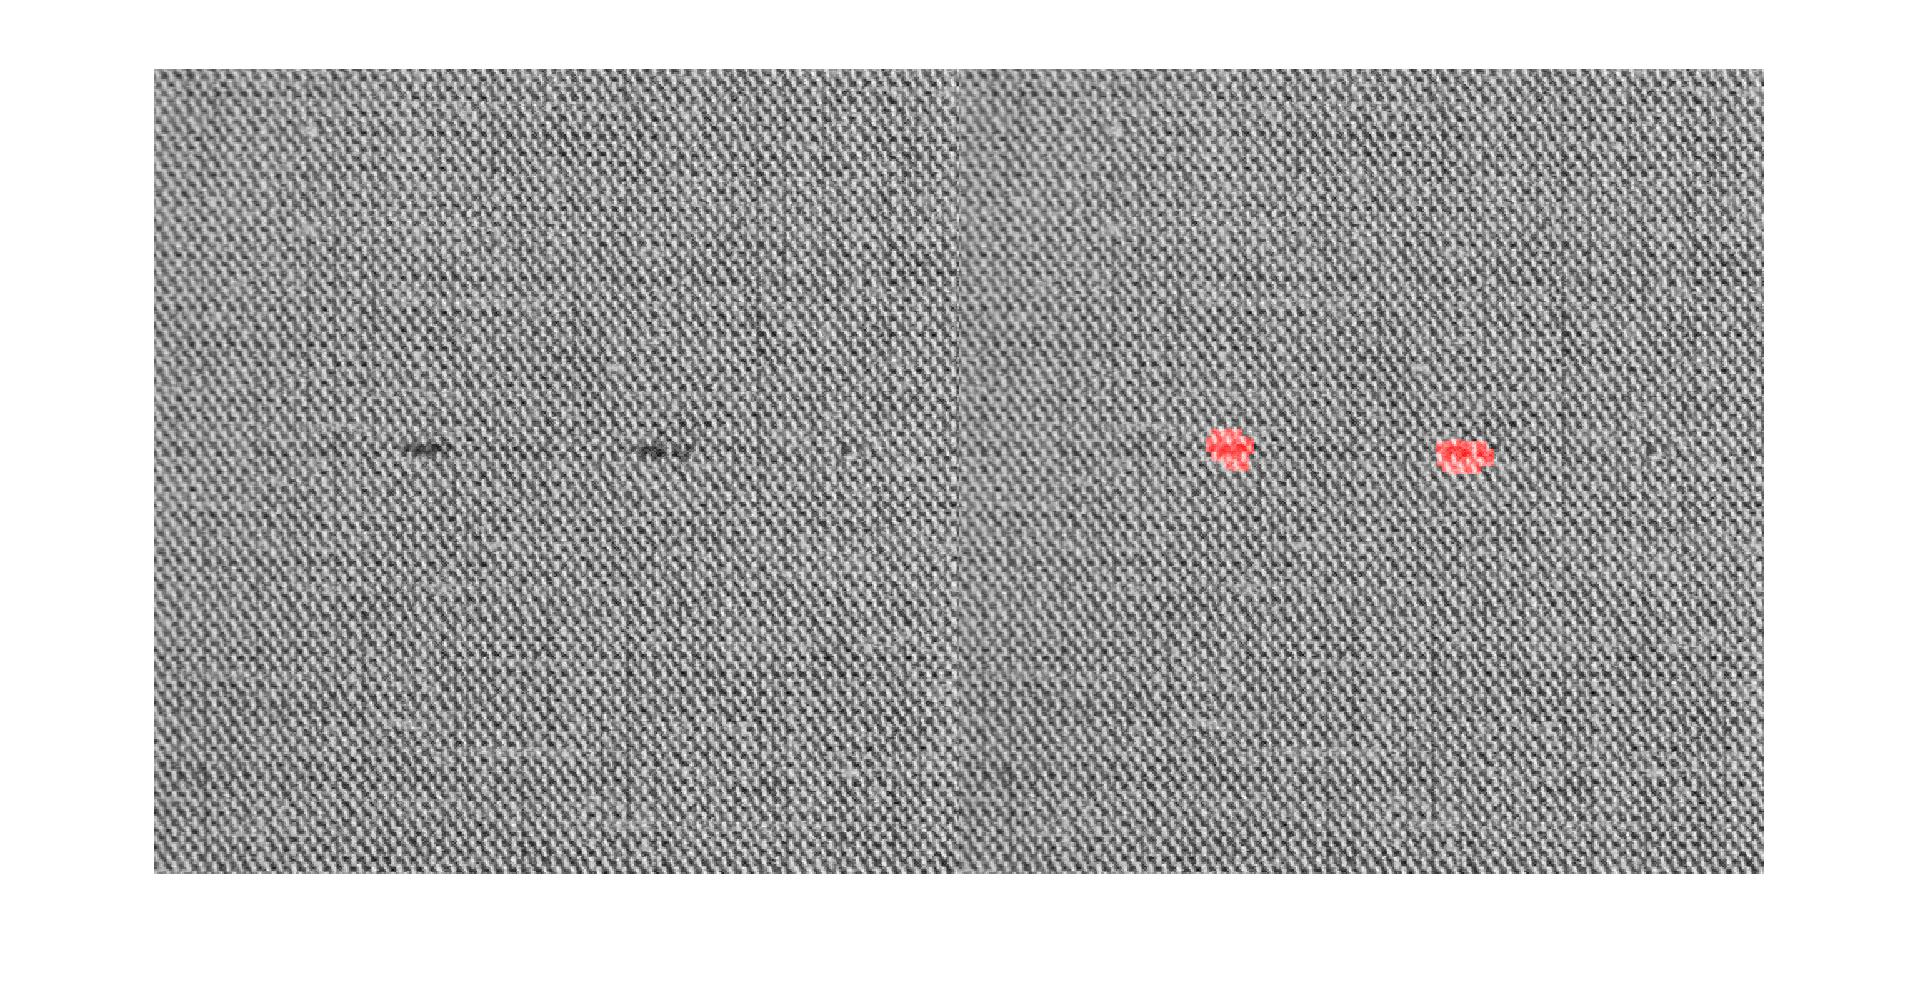
\includegraphics[width=\textwidth]{results/res1.jpg}
	\caption{Tessitura 1}
\end{figure}

\newpage

\subsection{Tessitura 2}

\begin{figure}[h!]
	\centering
	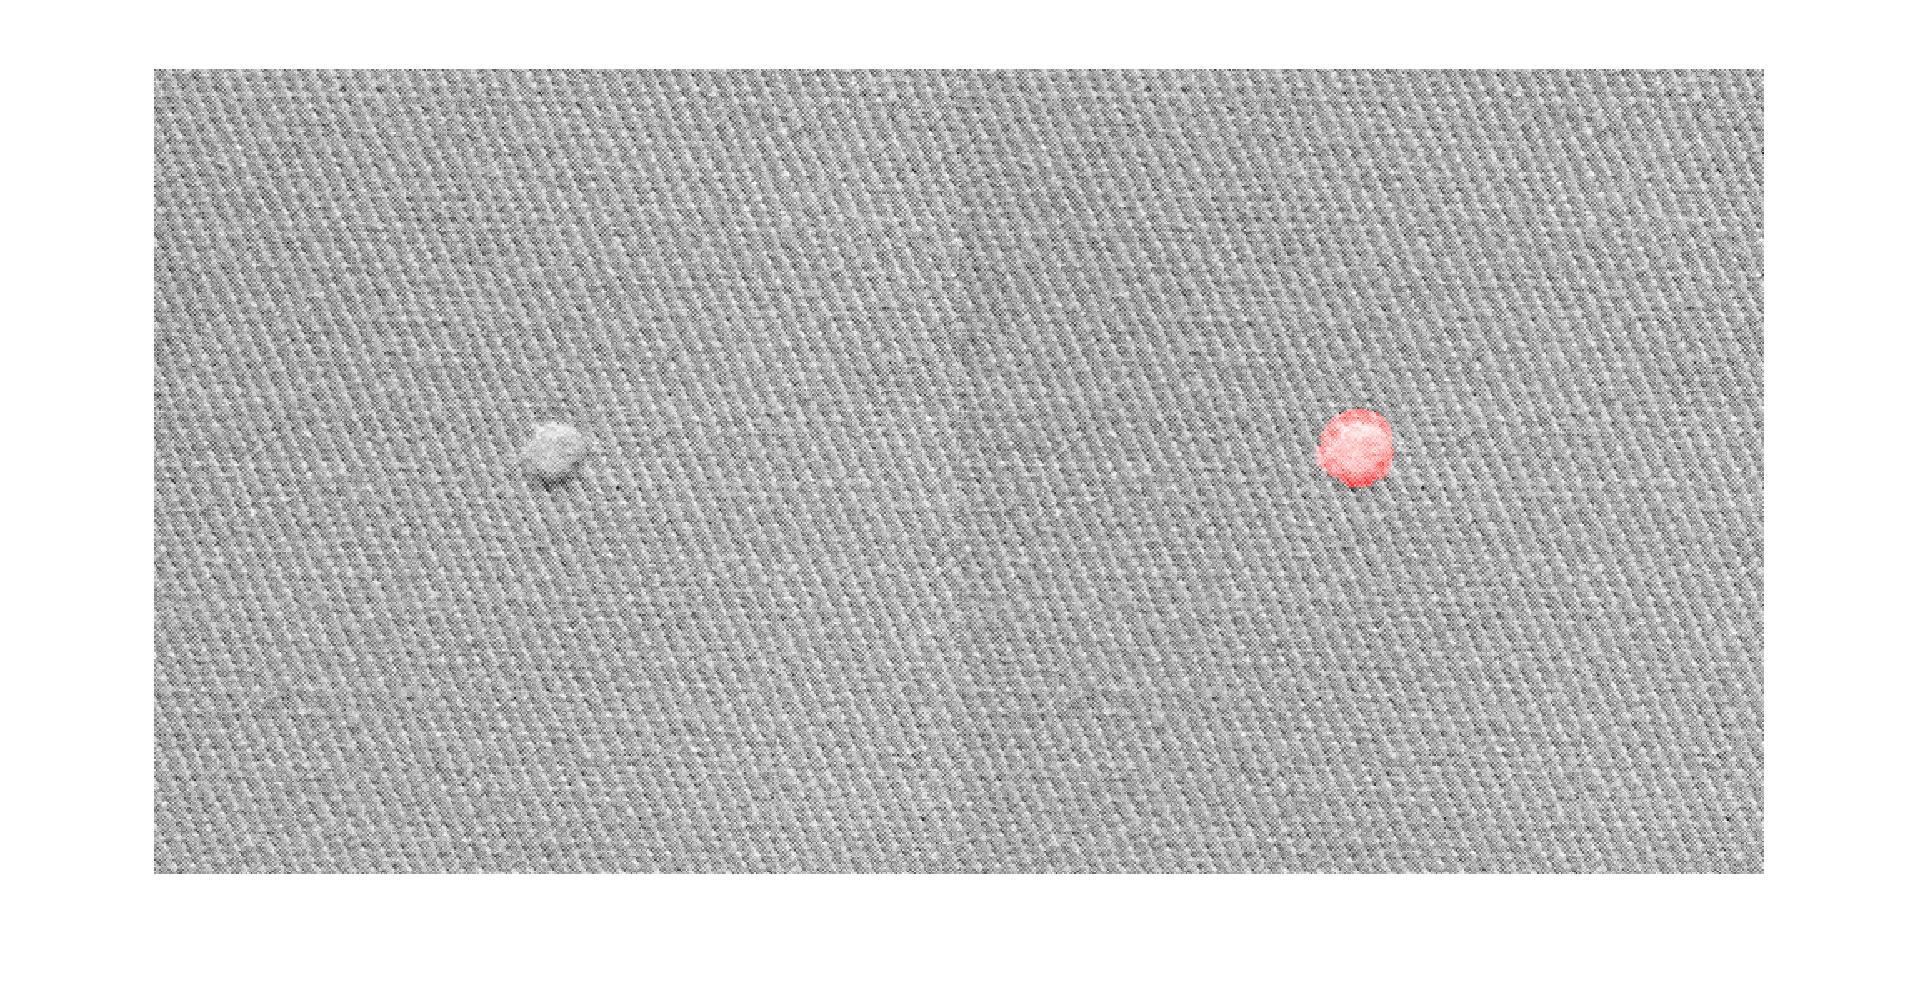
\includegraphics[width=\textwidth]{results/res2.jpg}
	\caption{Tessitura 2}
\end{figure}

\subsection{Tessitura 3}

\begin{figure}[h!]
	\centering
	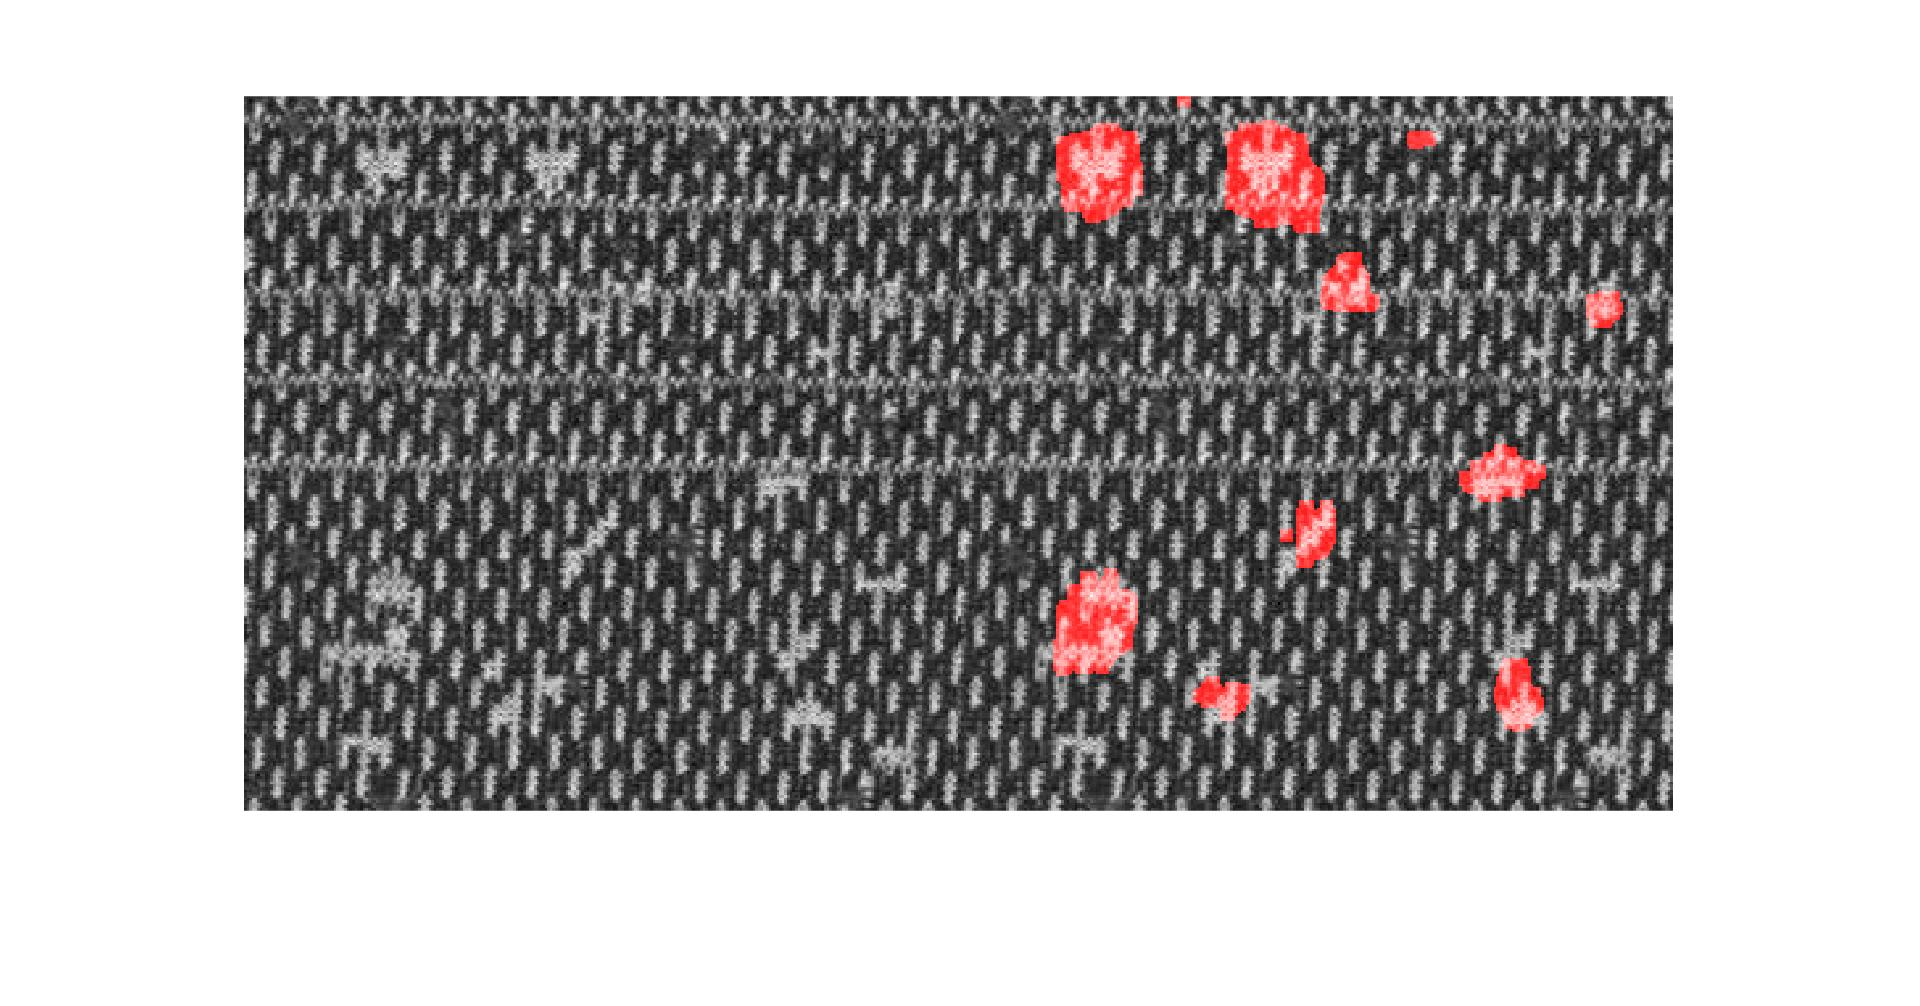
\includegraphics[width=\textwidth]{results/res3.jpg}
	\caption{Tessitura 3}
\end{figure}

In questo caso vengono individuate la maggior parte dei difetti ma non considera come difetti le righe che si trovano in alto alla figura(che per correttezza dovrebbero essere segnalate).

\subsection{Tessitura 4}

\begin{figure}[h!]
	\centering
	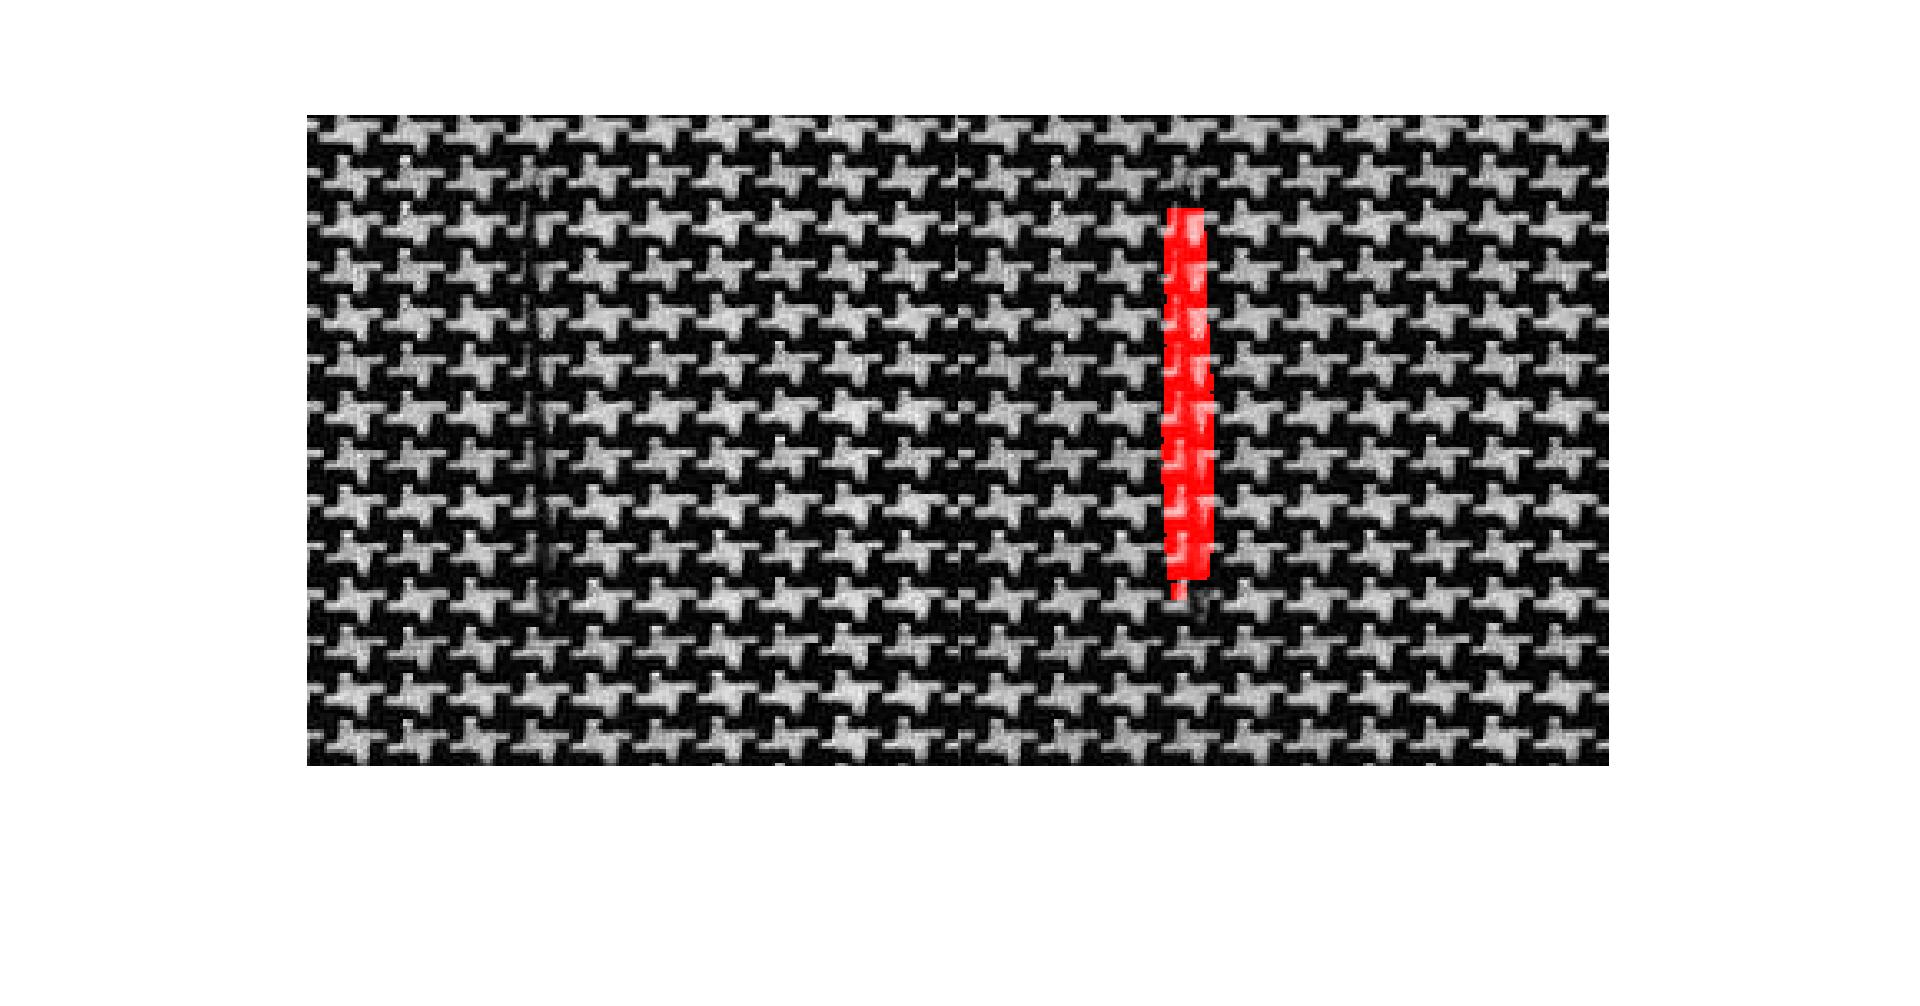
\includegraphics[width=\textwidth]{results/res4.jpg}
	\caption{Tessitura 4}
\end{figure}

Per ottenere questo risultato è stato necessario aumentare la dimensione dei quadrati dei pattern
in modo che racchiudano il disegno (pied-de-poule) che si ripete in tutta la tessitura.

\subsection{Tessitura 5}

\begin{figure}[h!]
	\centering
	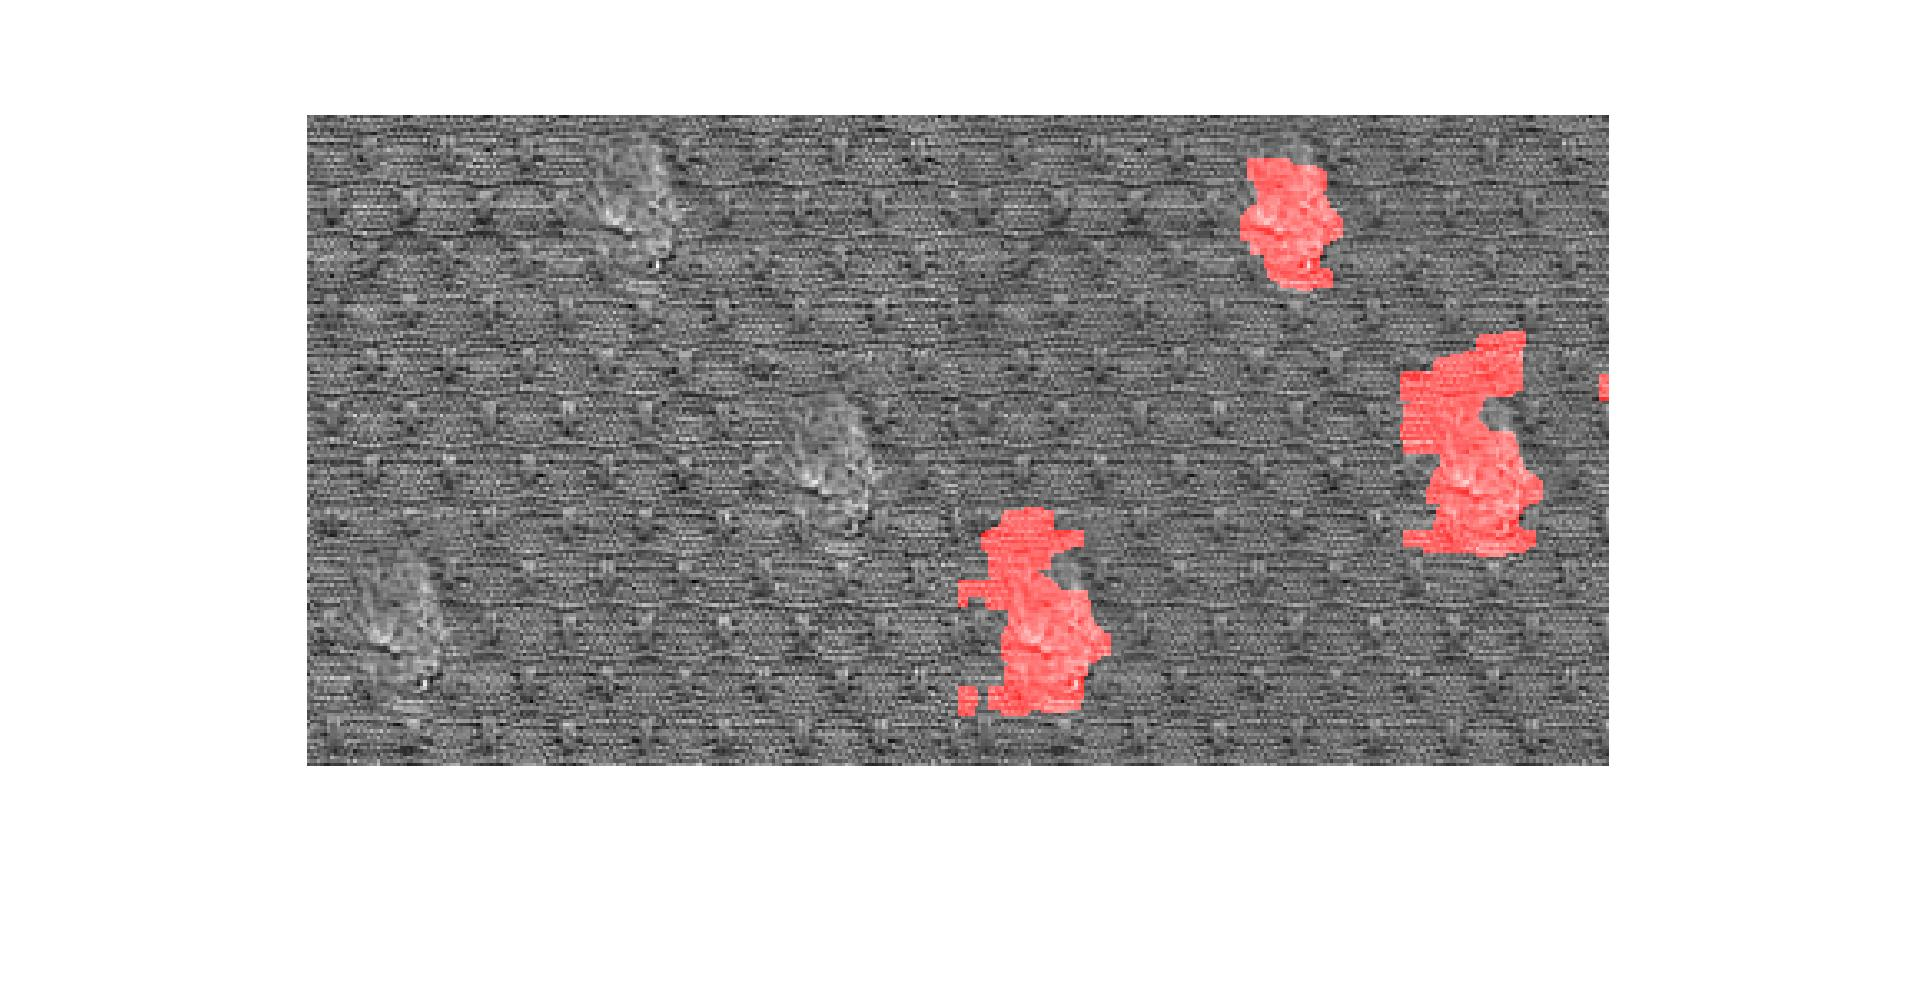
\includegraphics[width=\textwidth]{results/res5.jpg}
	\caption{Tessitura 5}
\end{figure}

\subsection{Tessitura 6}

\begin{figure}[h!]
	\centering
	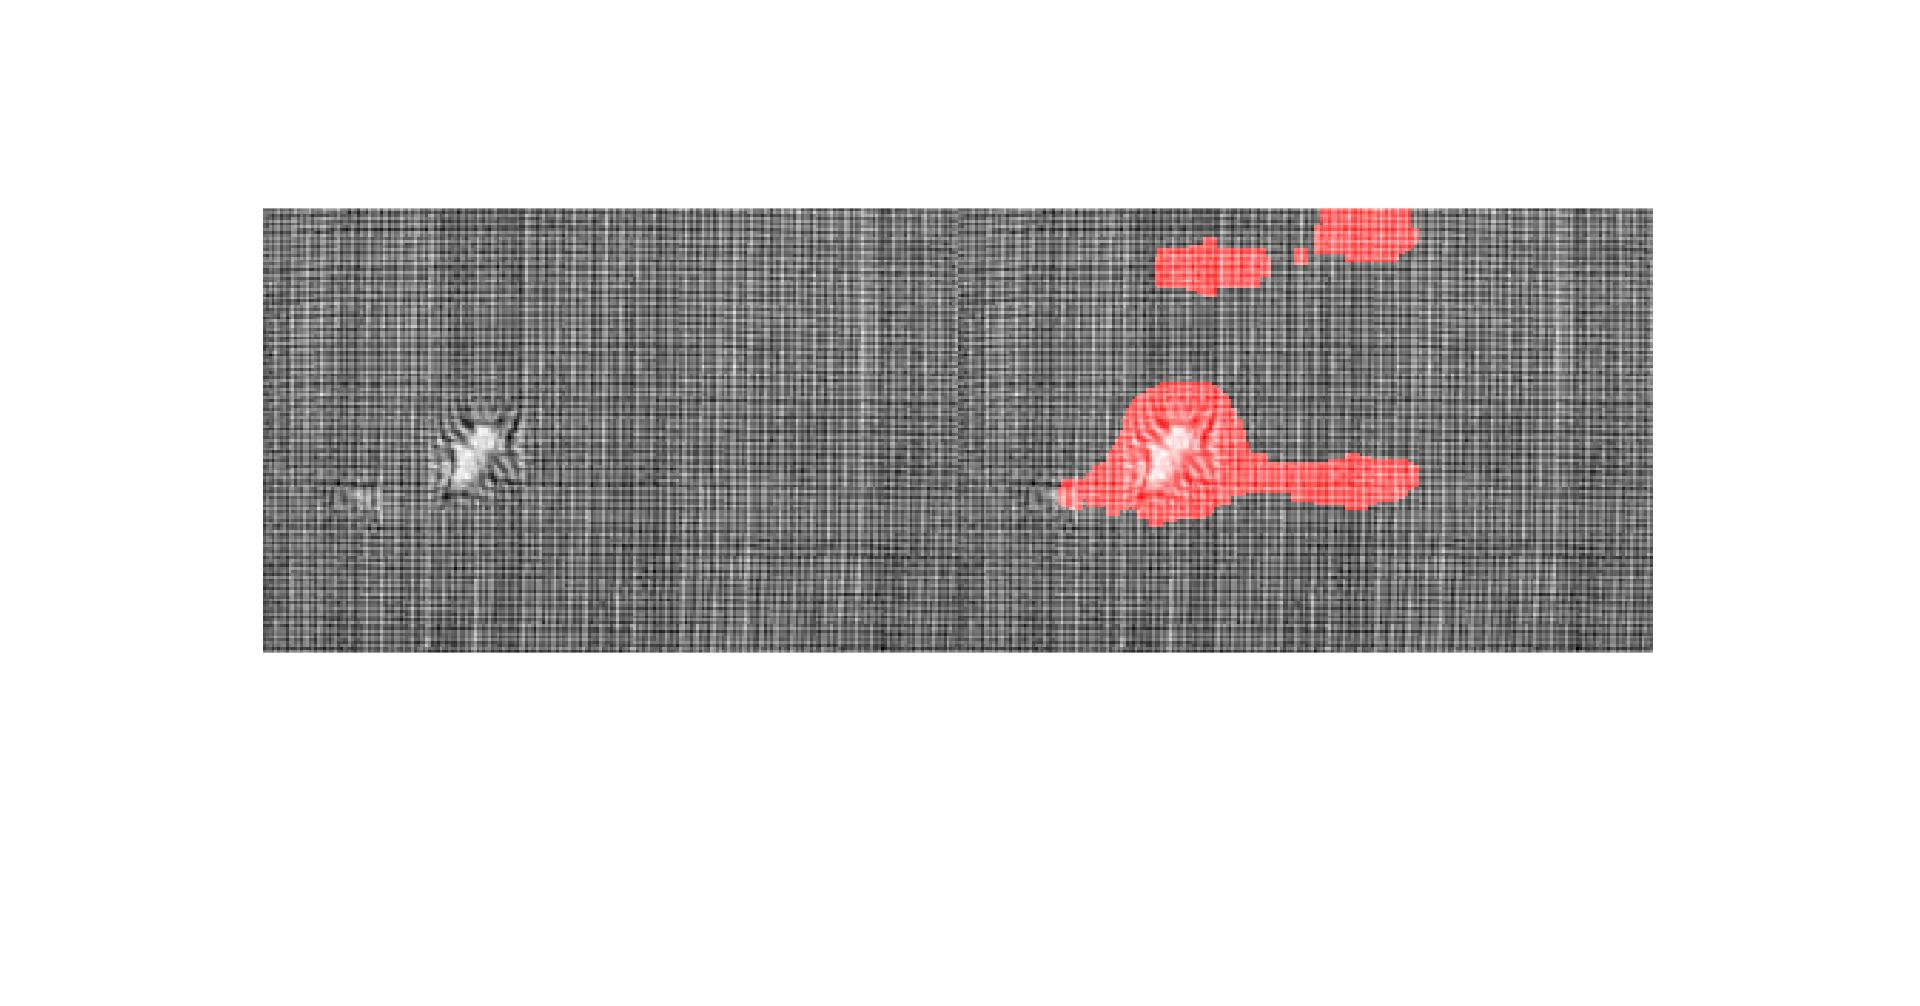
\includegraphics[width=\textwidth]{results/res6.jpg}
	\caption{Tessitura 6}
\end{figure}

\subsection{Tessitura 7}

\begin{figure}[h!]
	\centering
	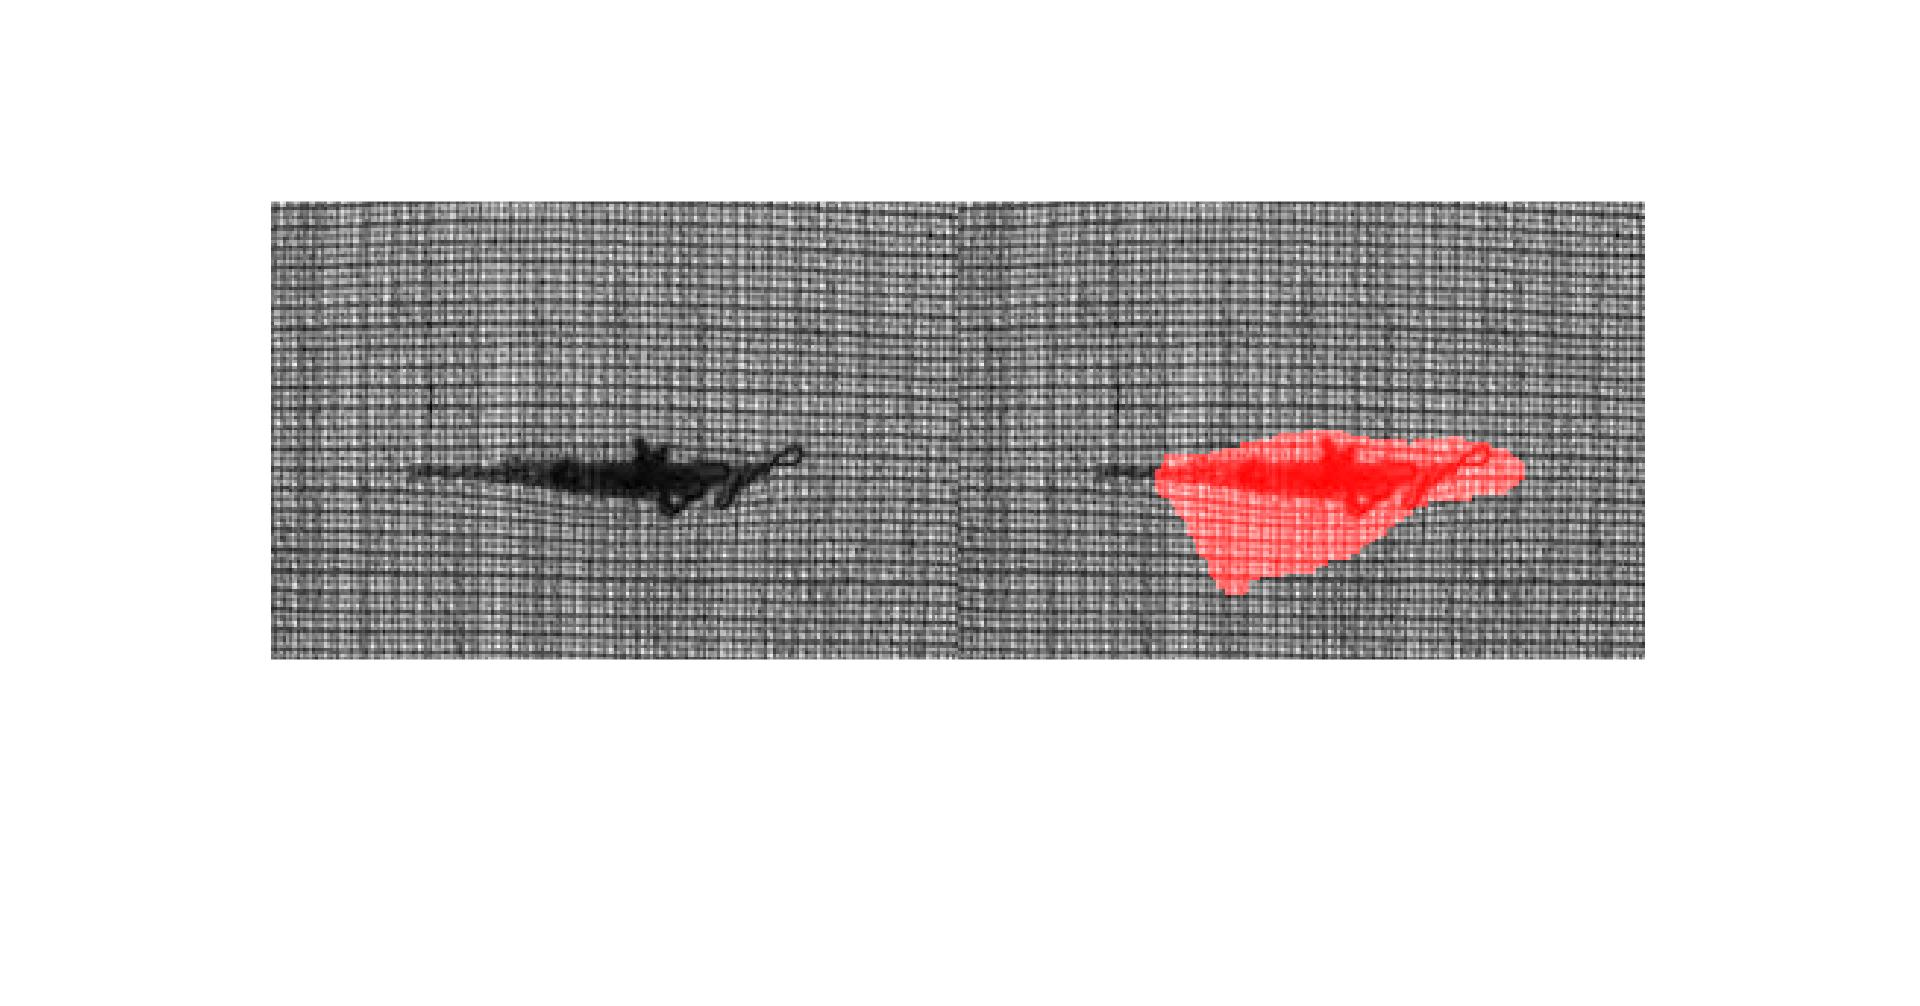
\includegraphics[width=\textwidth]{results/res7.jpg}
	\caption{Tessitura 7}
\end{figure}

\newpage

\subsection{Tessitura 8}

\begin{figure}[h!]
	\centering
	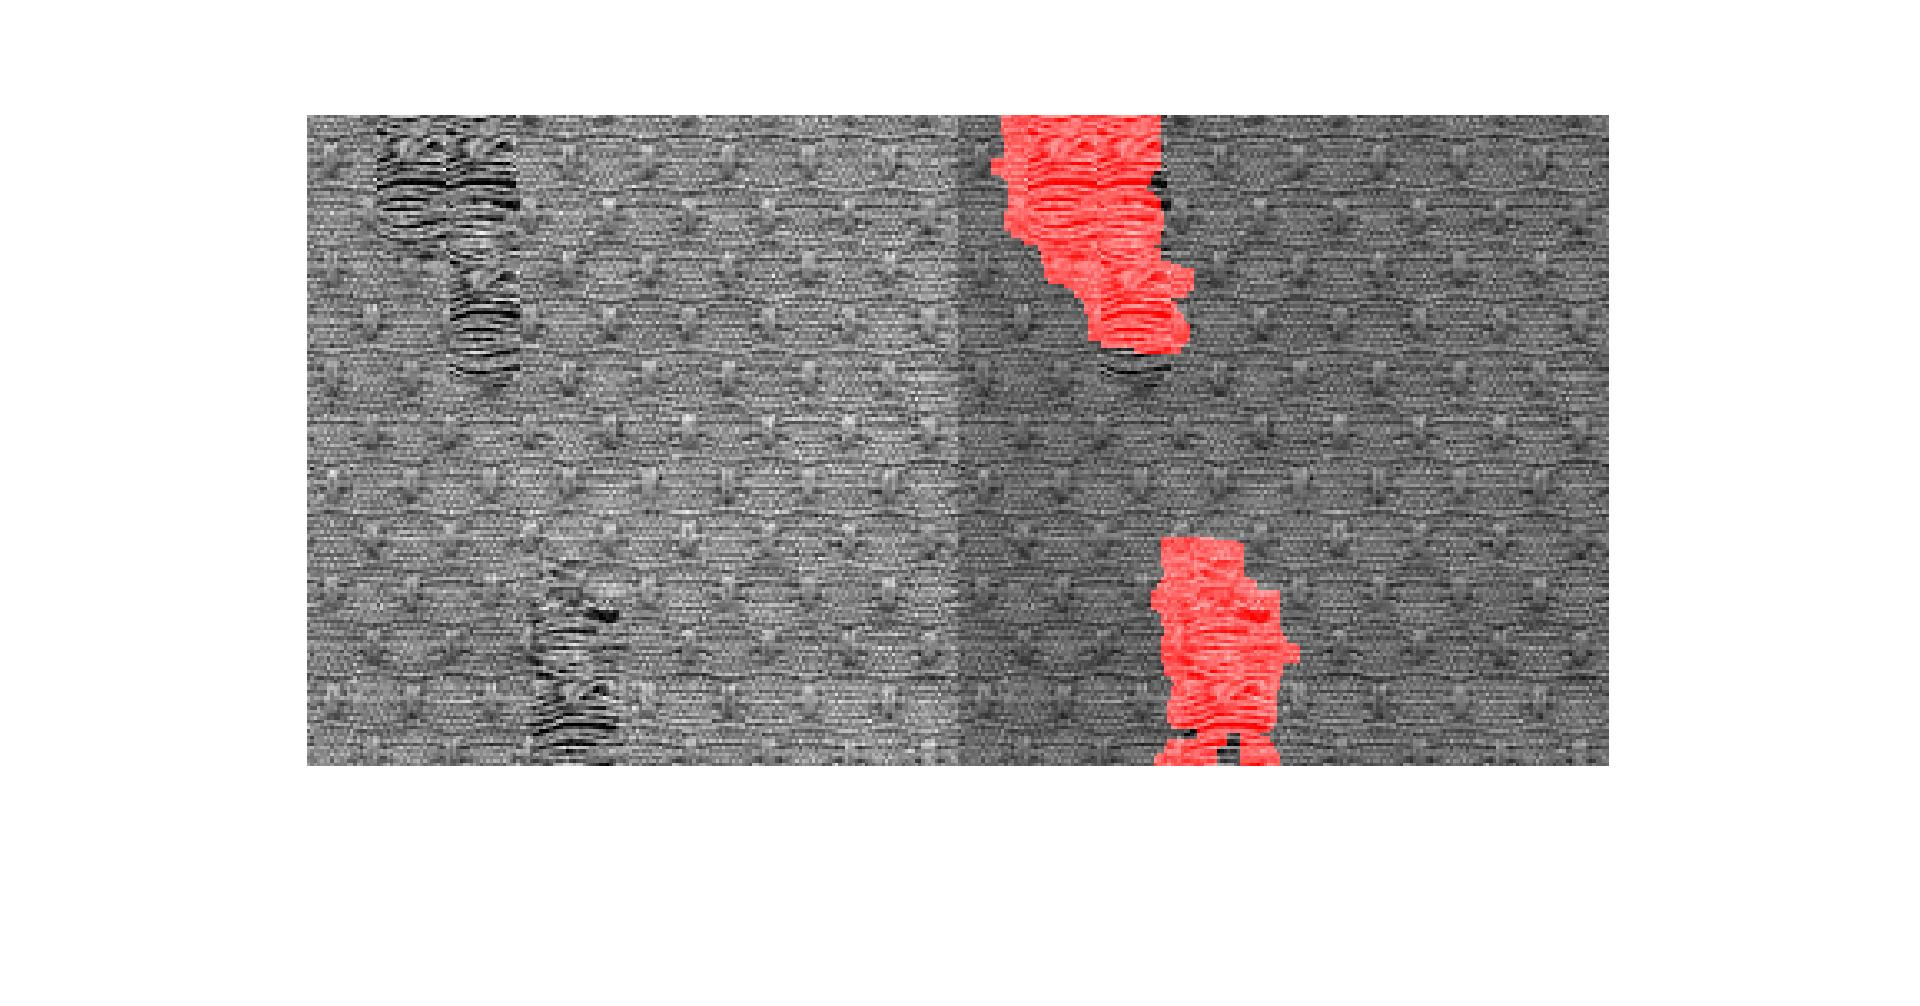
\includegraphics[width=\textwidth]{results/res8.jpg}
	\caption{Tessitura 8}
\end{figure}

\subsection{Tessitura 9}

\begin{figure}[h!]
	\centering
	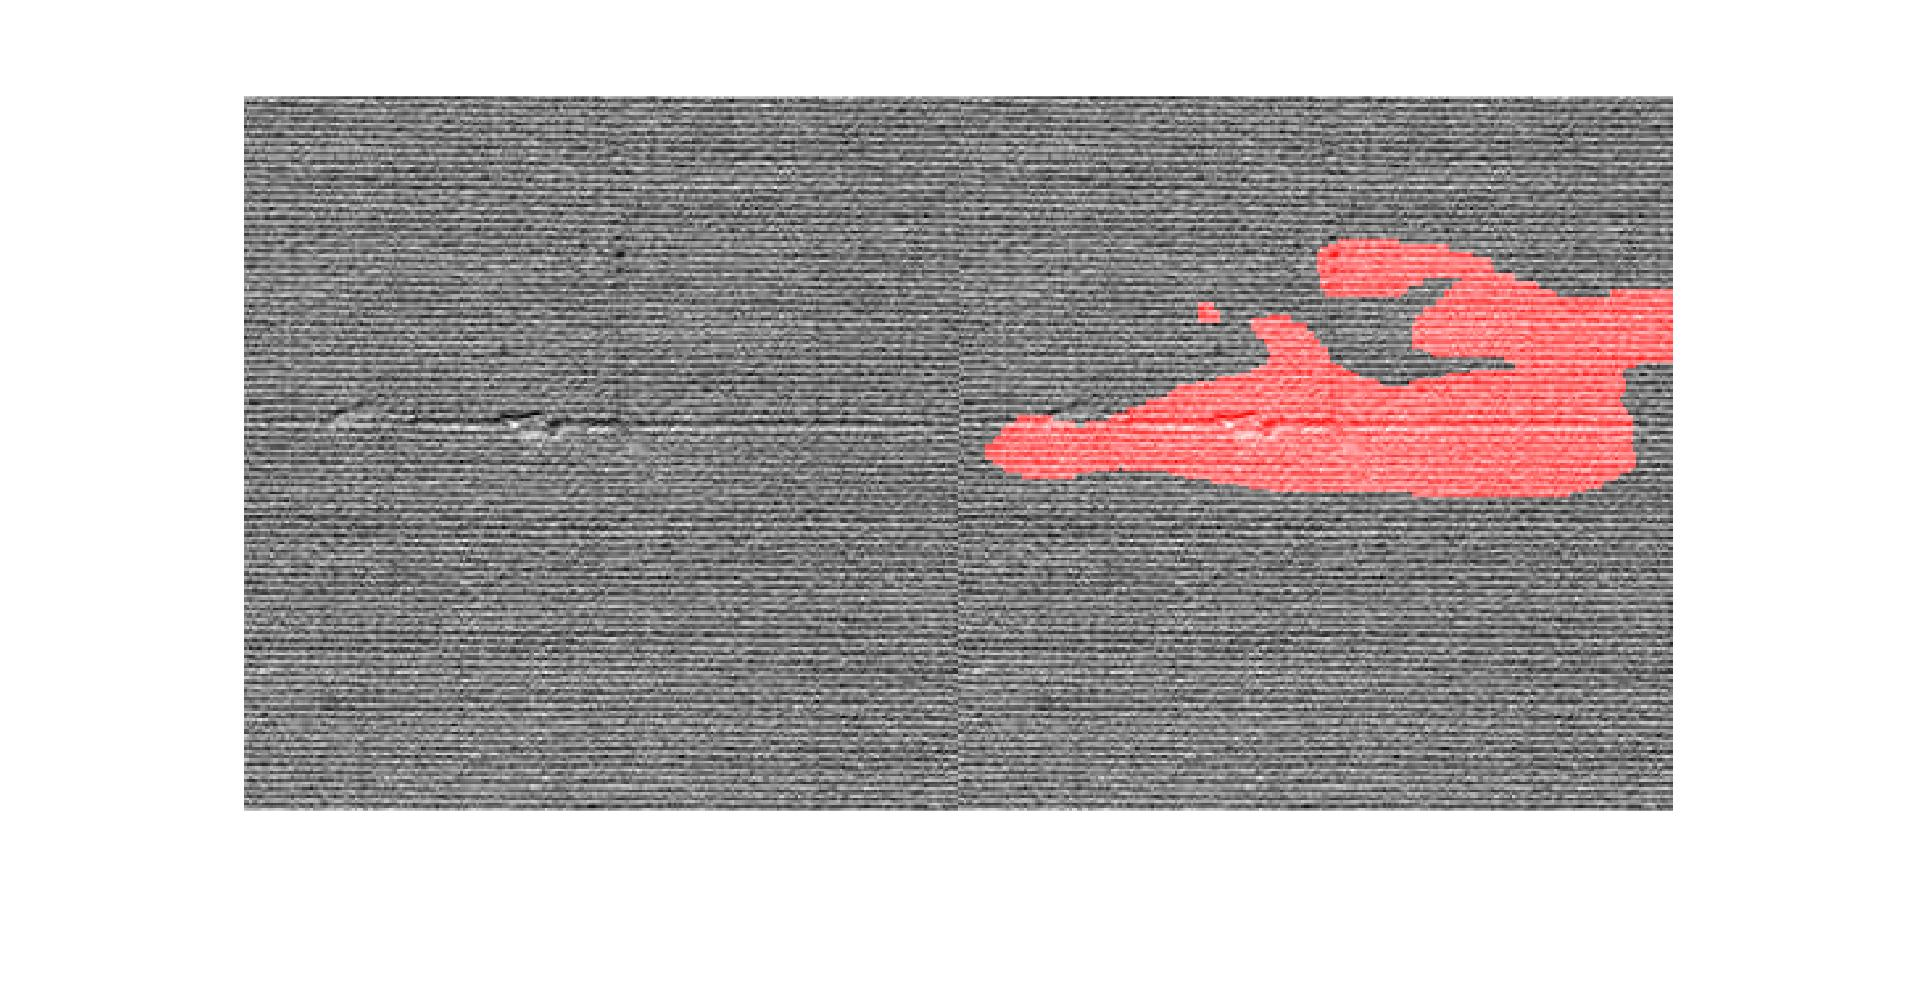
\includegraphics[width=\textwidth]{results/res9.jpg}
	\caption{Tessitura 9}
\end{figure}

\newpage

\subsection{Tessitura 10}

\begin{figure}[h!]
	\centering
	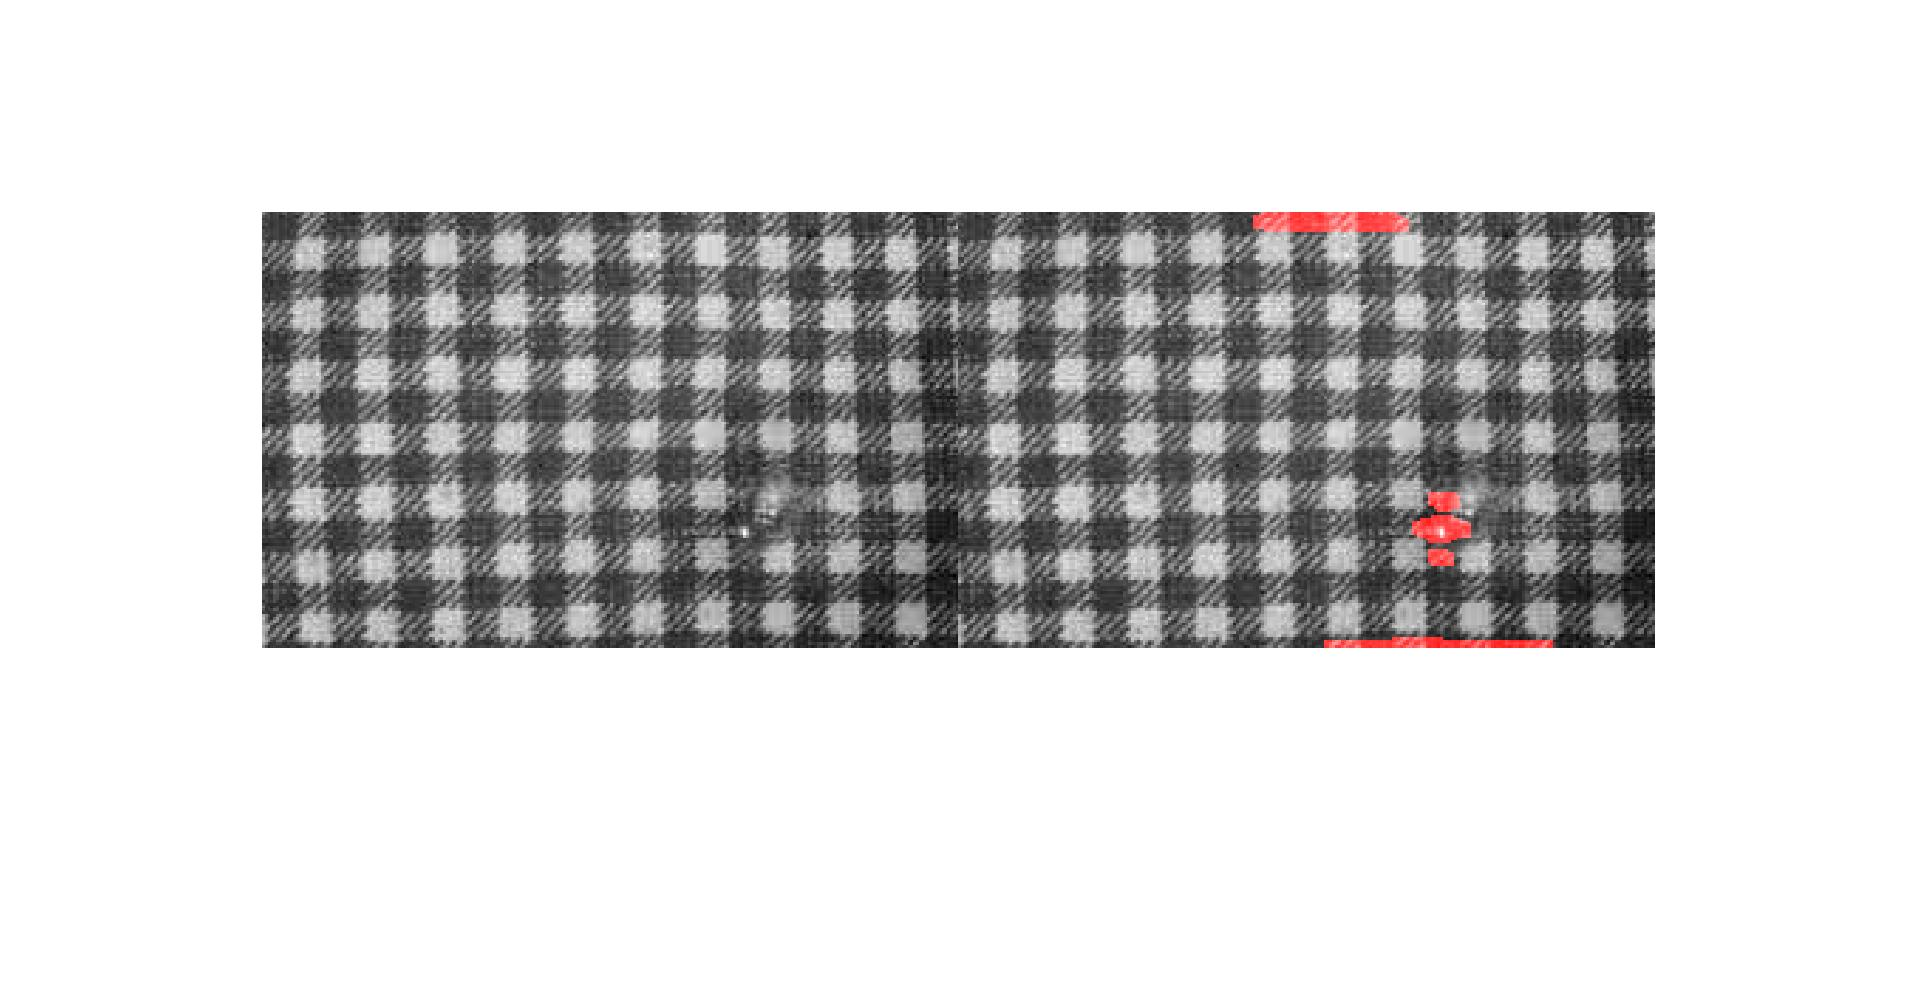
\includegraphics[width=\textwidth]{results/res10.jpg}
	\caption{Tessitura 10}
\end{figure}

Problema simile a quello della tessitura 4.

\subsection{Tessitura 11}

\begin{figure}[h!]
	\centering
	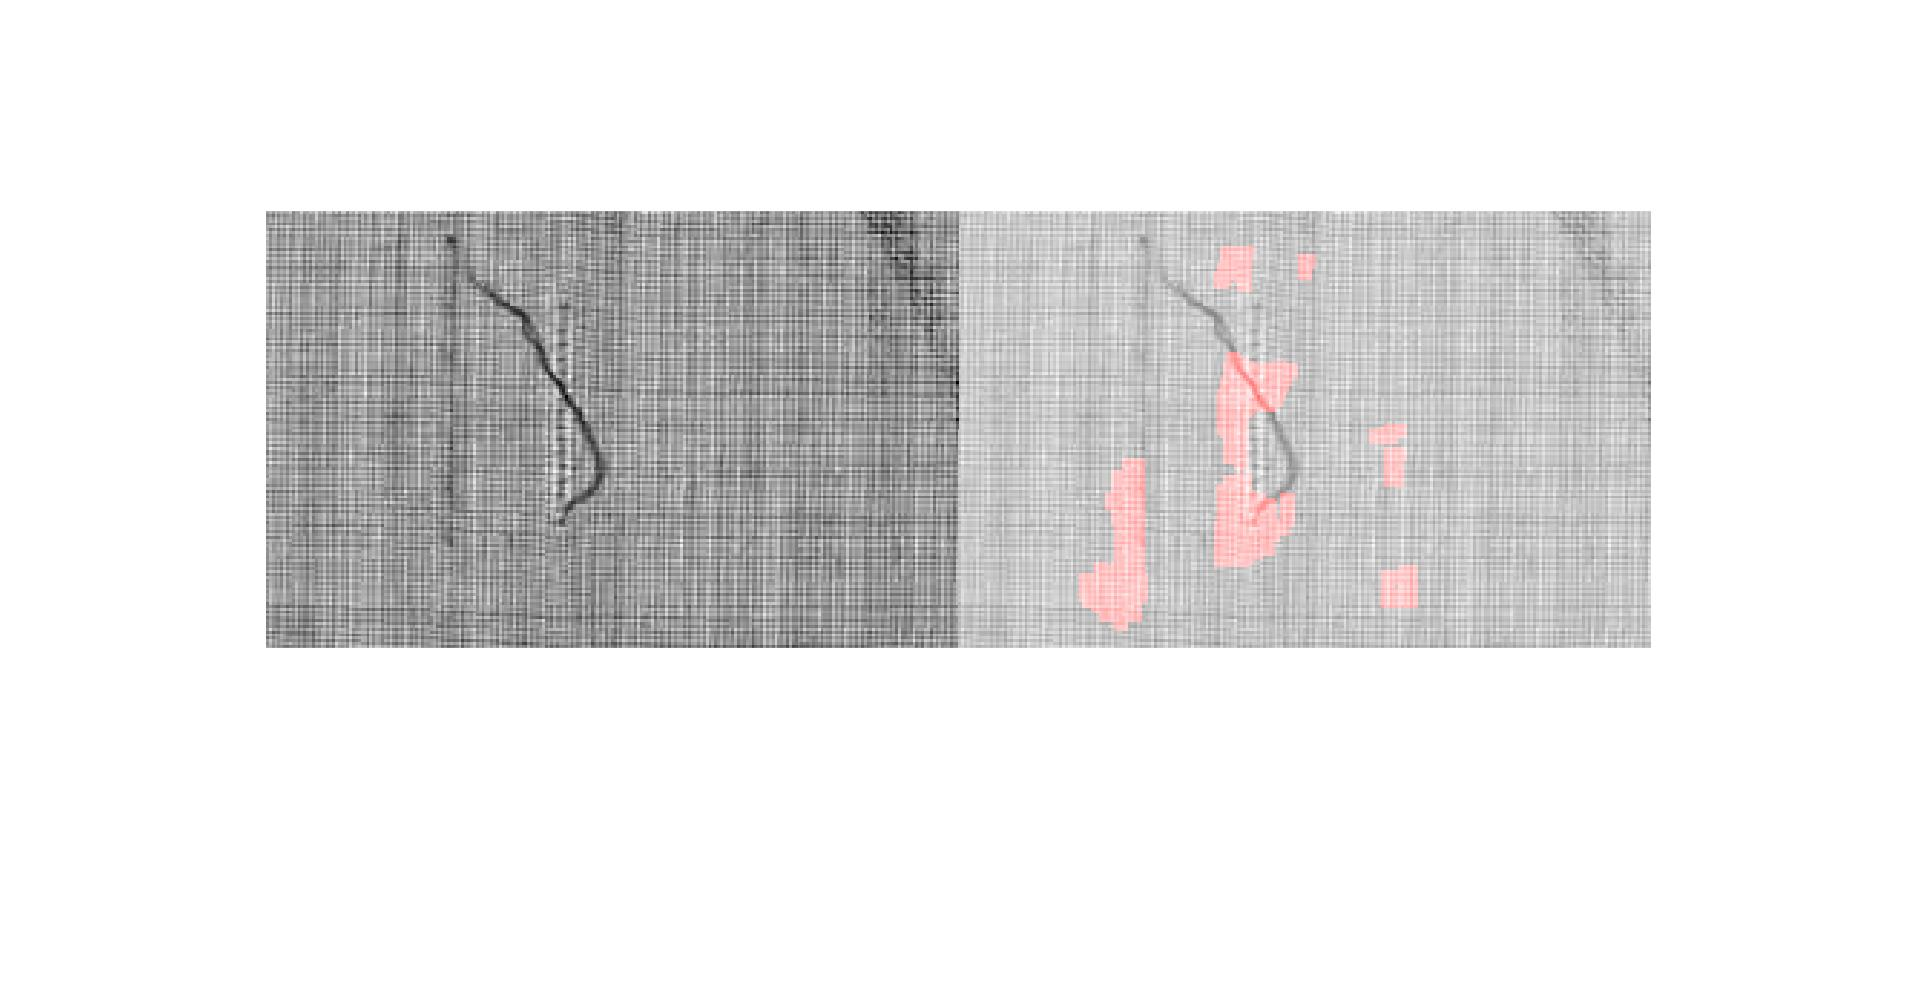
\includegraphics[width=\textwidth]{results/res11.jpg}
	\caption{Tessitura 11}
\end{figure}

Nella seguente tessitura vengono individuati buona parte dei difetti, ma risulta mancante l'evidenziazione del filo nero e una parte del buco centrale forse questa mancanza è data dall'angolo in alto a destra che risulta più scuro.

\subsection{Tessitura 12}

\begin{figure}[h!]
	\centering
	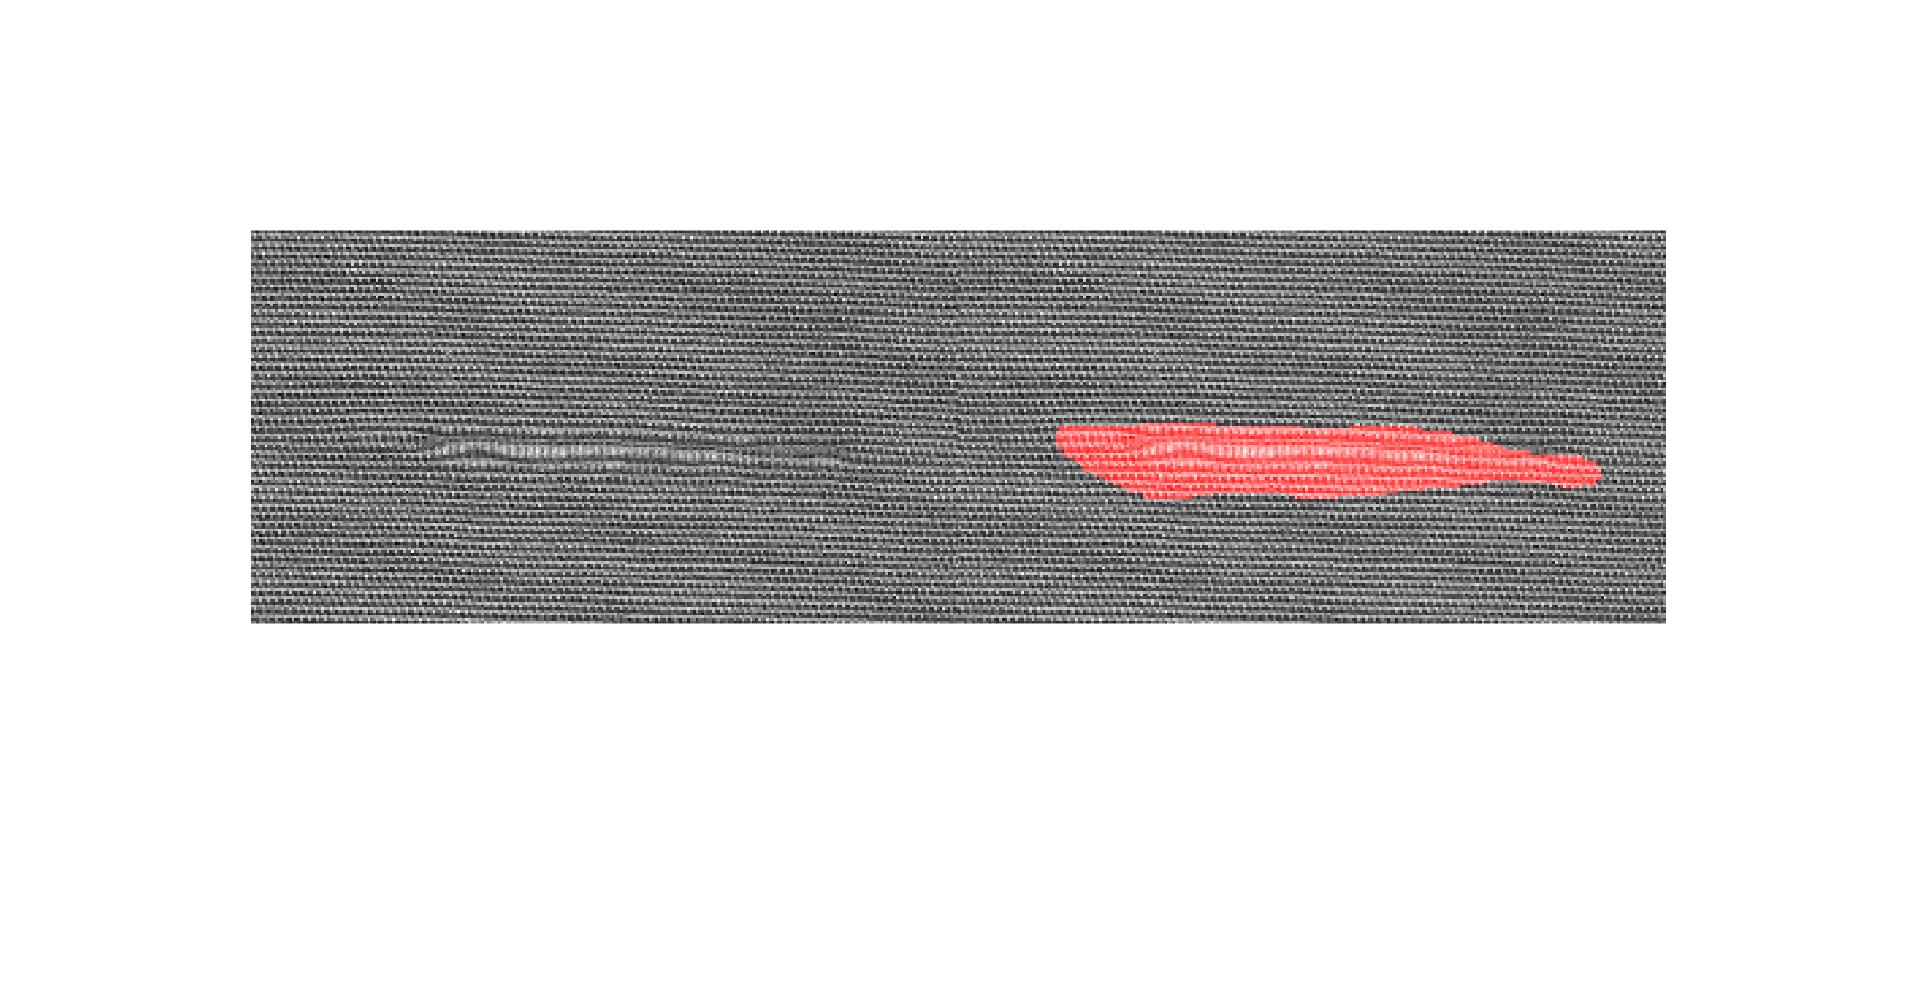
\includegraphics[width=\textwidth]{results/res12.jpg}
	\caption{Tessitura 12}
\end{figure}

\subsection{Tessitura 13}

\begin{figure}[h!]
	\centering
	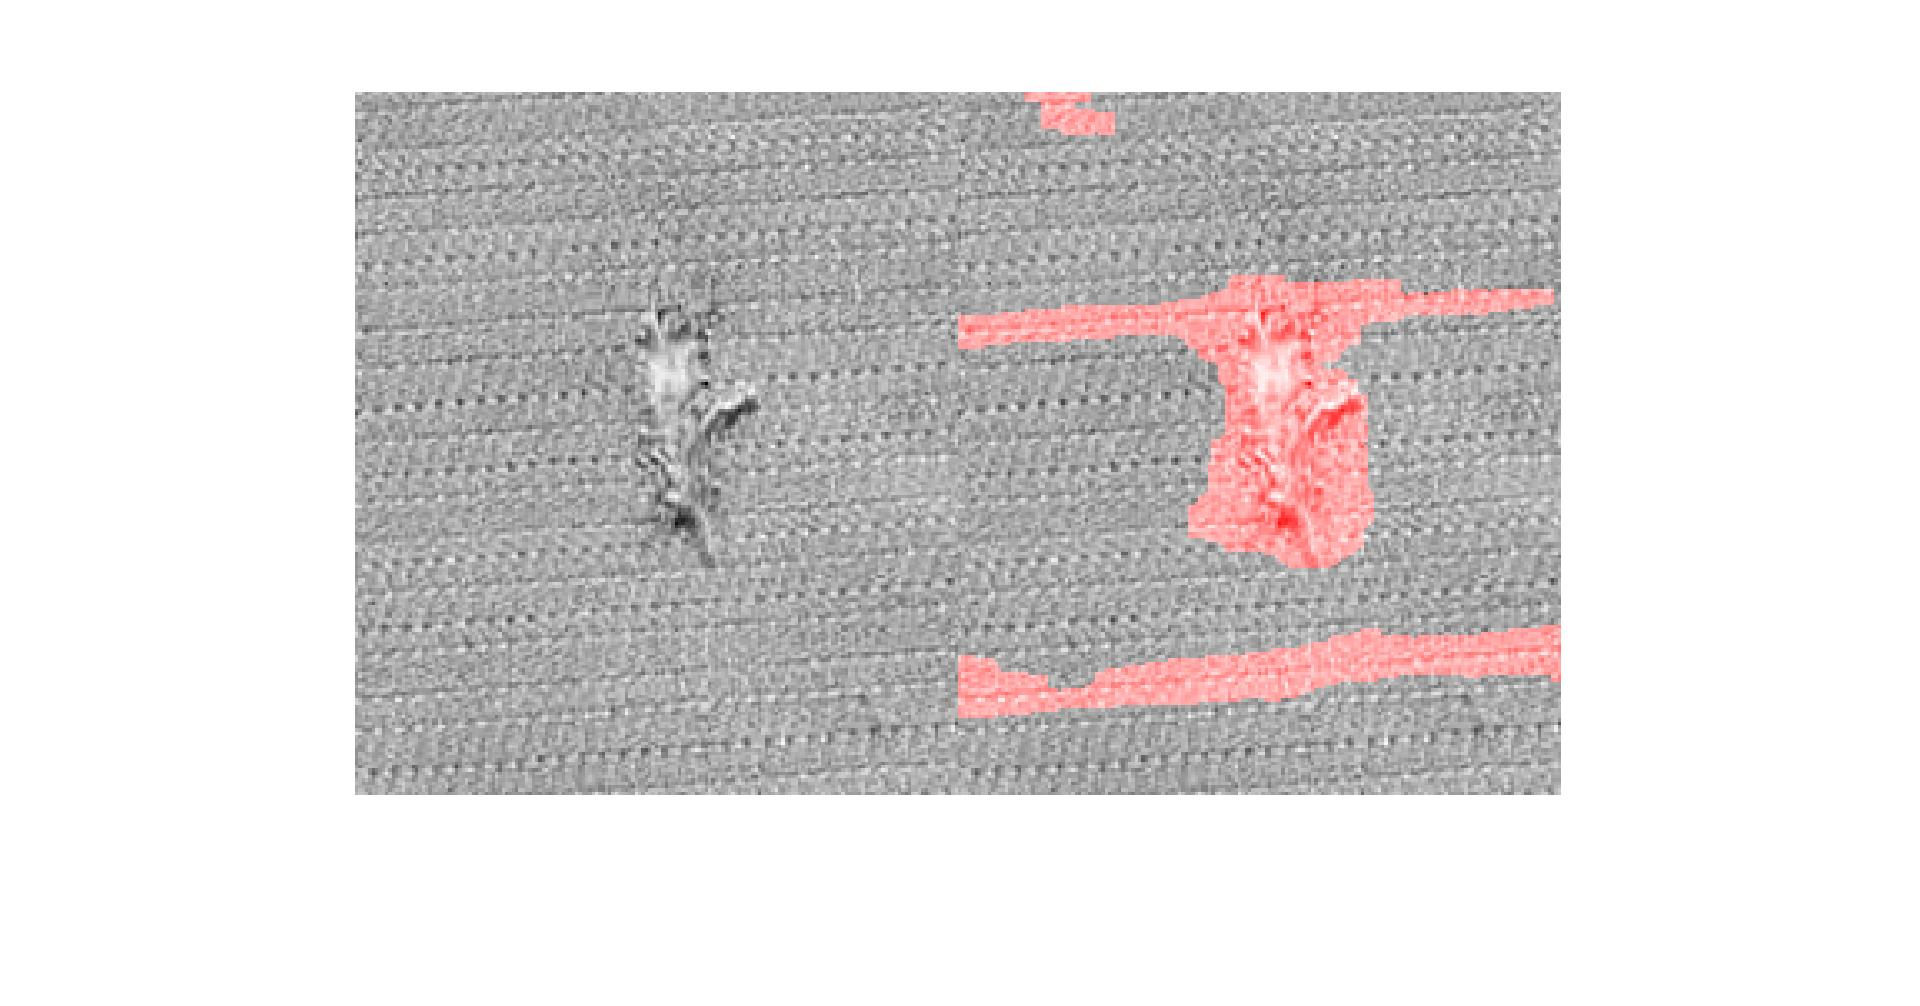
\includegraphics[width=\textwidth]{results/res13.jpg}
	\caption{Tessitura 13}
\end{figure}

\newpage

\subsection{Tessitura 14}

\begin{figure}[h!]
	\centering
	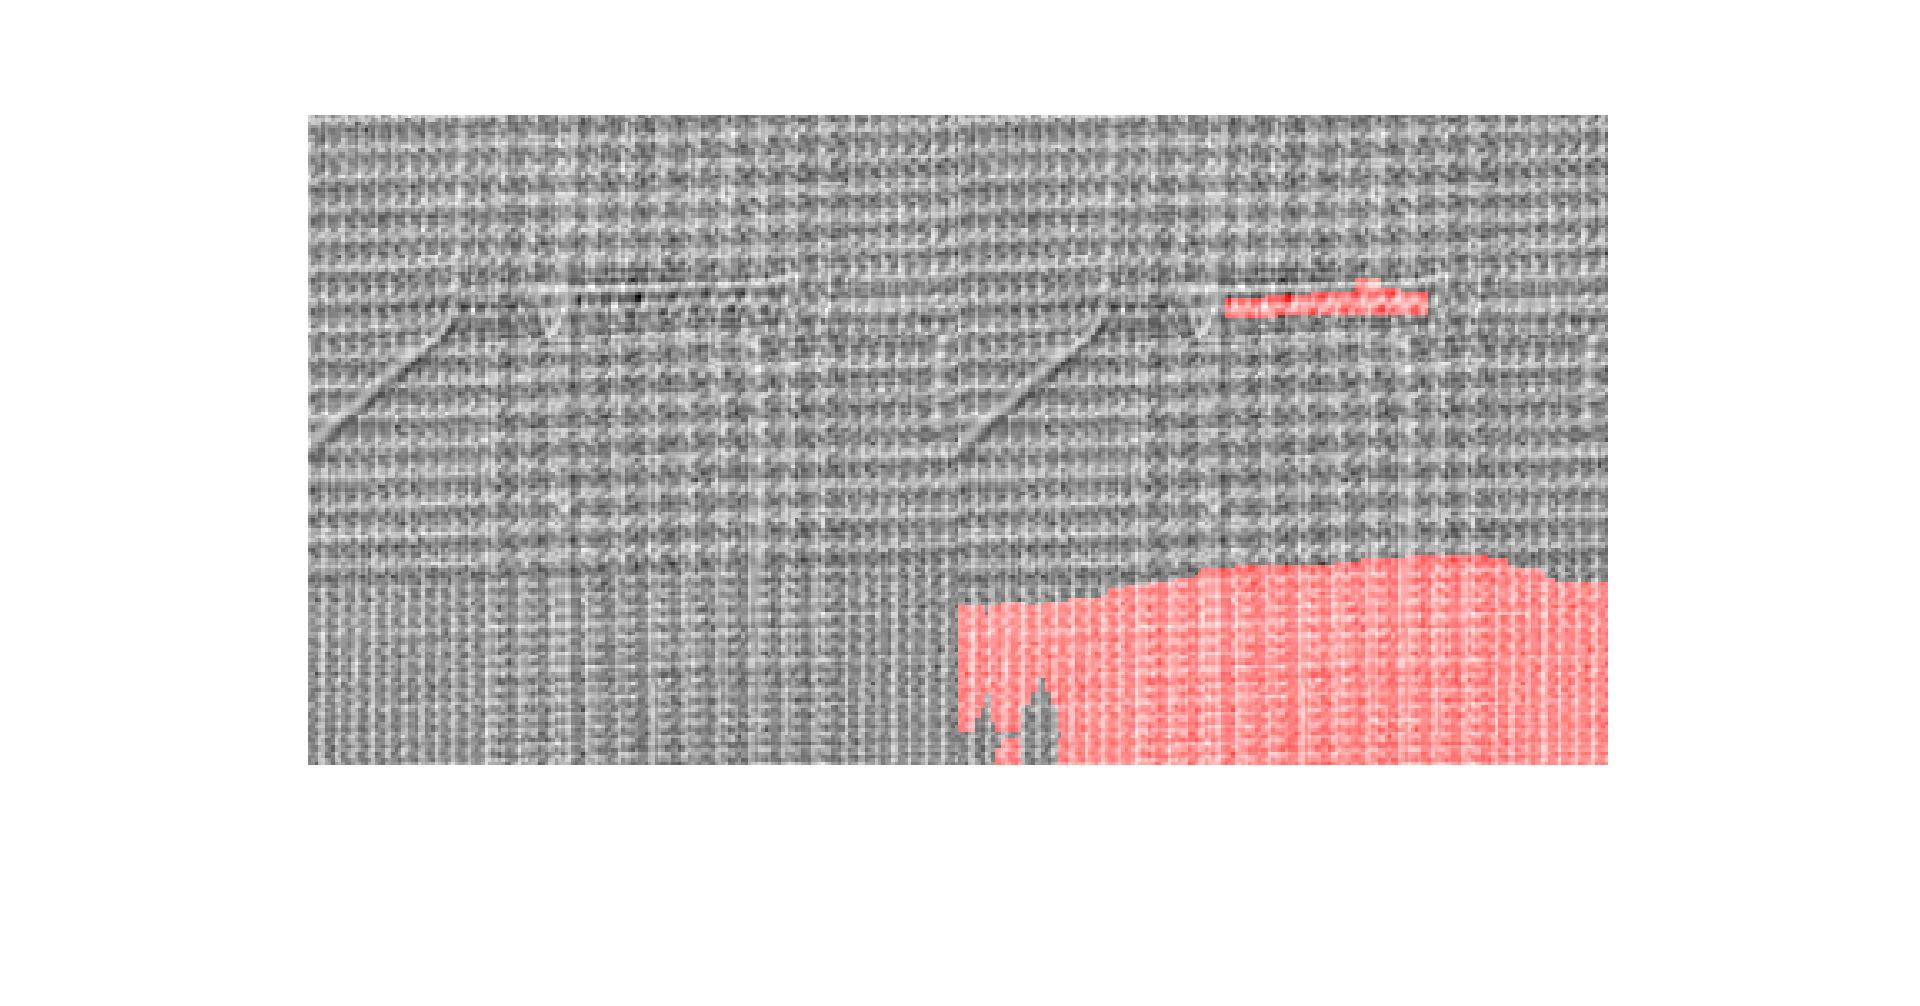
\includegraphics[width=\textwidth]{results/res14.jpg}
	\caption{Tessitura 14}
\end{figure}

L'immagine seguente presenta due difetti uno dato dal filo scucito che però non viene evidenziato mentre l'altro che si trova in basso dove la tessitura risulta essere più tesa non viene del tutto evidenziato.

\newpage

\subsection{Tessitura 15}

\begin{figure}[h!]
	\centering
	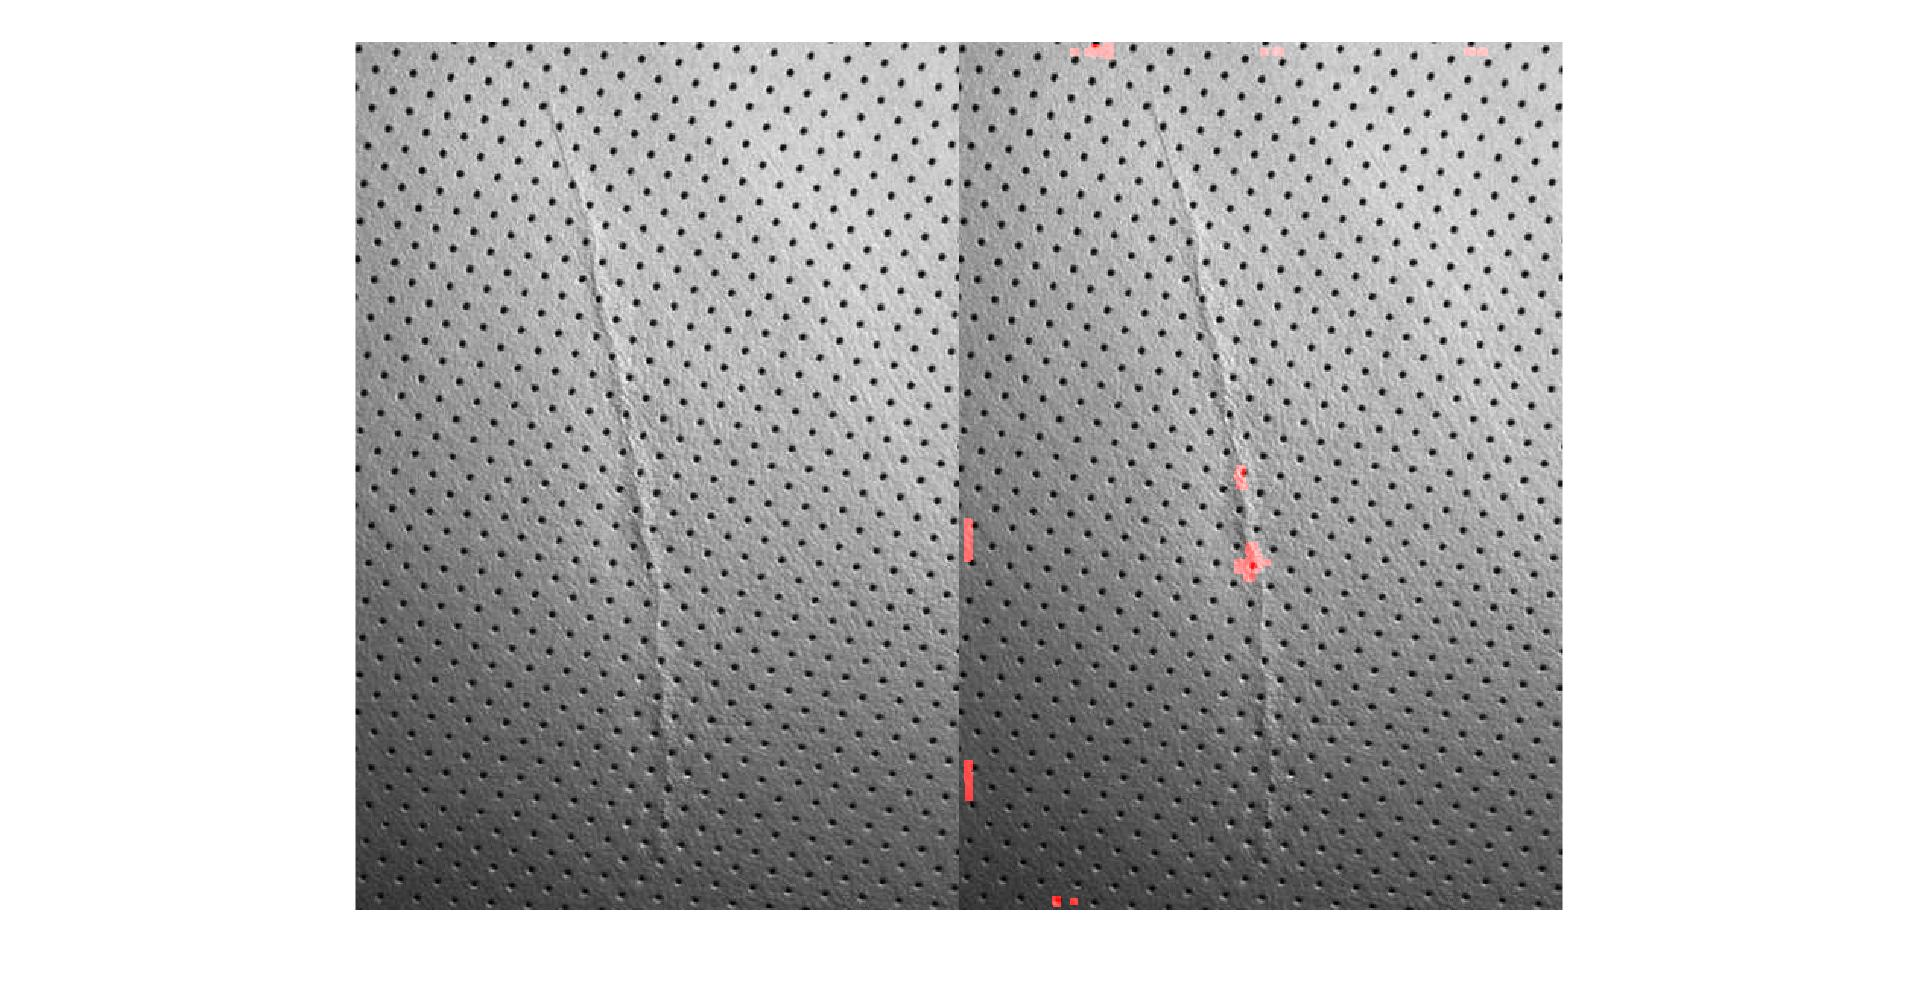
\includegraphics[width=\textwidth]{results/res15.jpg}
	\caption{Tessitura 15}
	
\end{figure}

La seguente immagine rappresenta un particolare tipo di tessuto ovvero pelle con dei fori. Il metodo per l'individuazione dei difetti da noi sviluppato non si adatta a questa tipologia di immagini, probabilmente per due motivi, uno dei quali legato alla colorazione dell'immagine infatti in alto risulta più chiara mentre in basso è più scura invece l'altro forse è dato dal pattern bucherellato.

\newpage

\subsection{Tessitura 16}

\begin{figure}[h!]
	\centering
	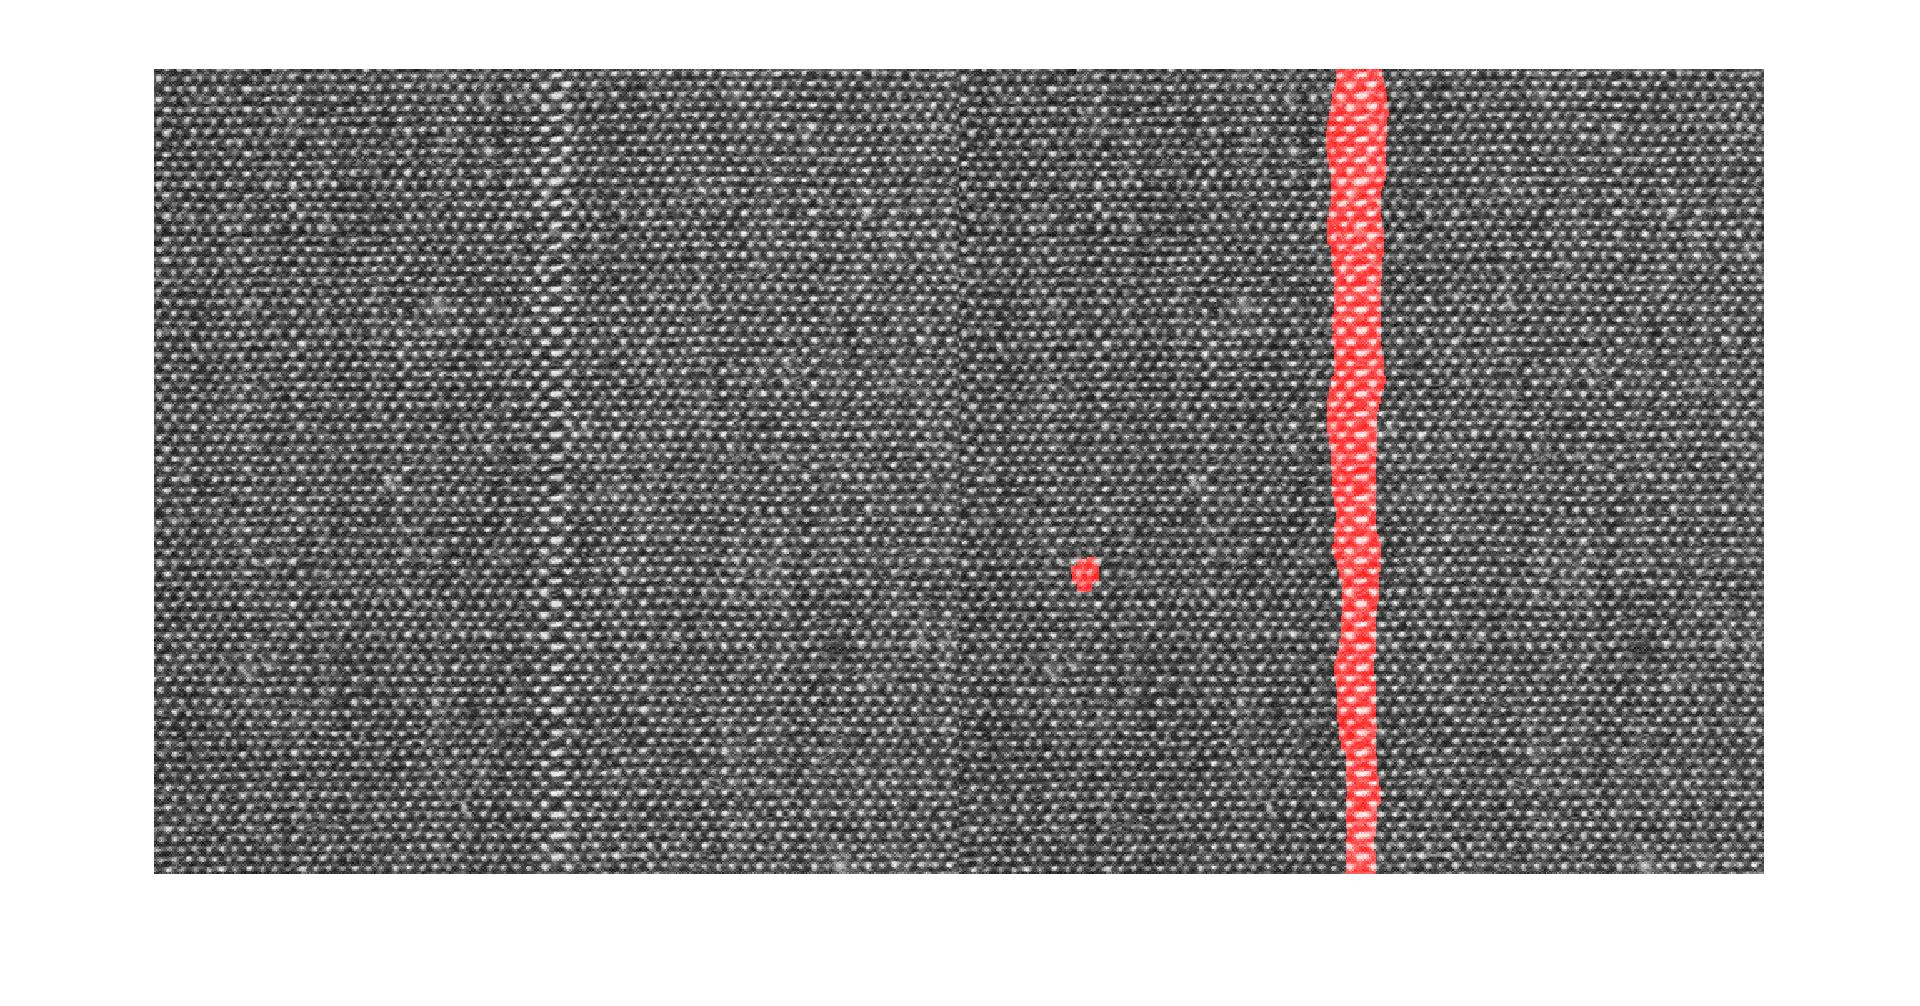
\includegraphics[width=\textwidth]{results/res16.jpg}
	\caption{Tessitura 16}
\end{figure}

\newpage

\subsection{Tessitura 17}

\begin{figure}[h!]
	\centering
	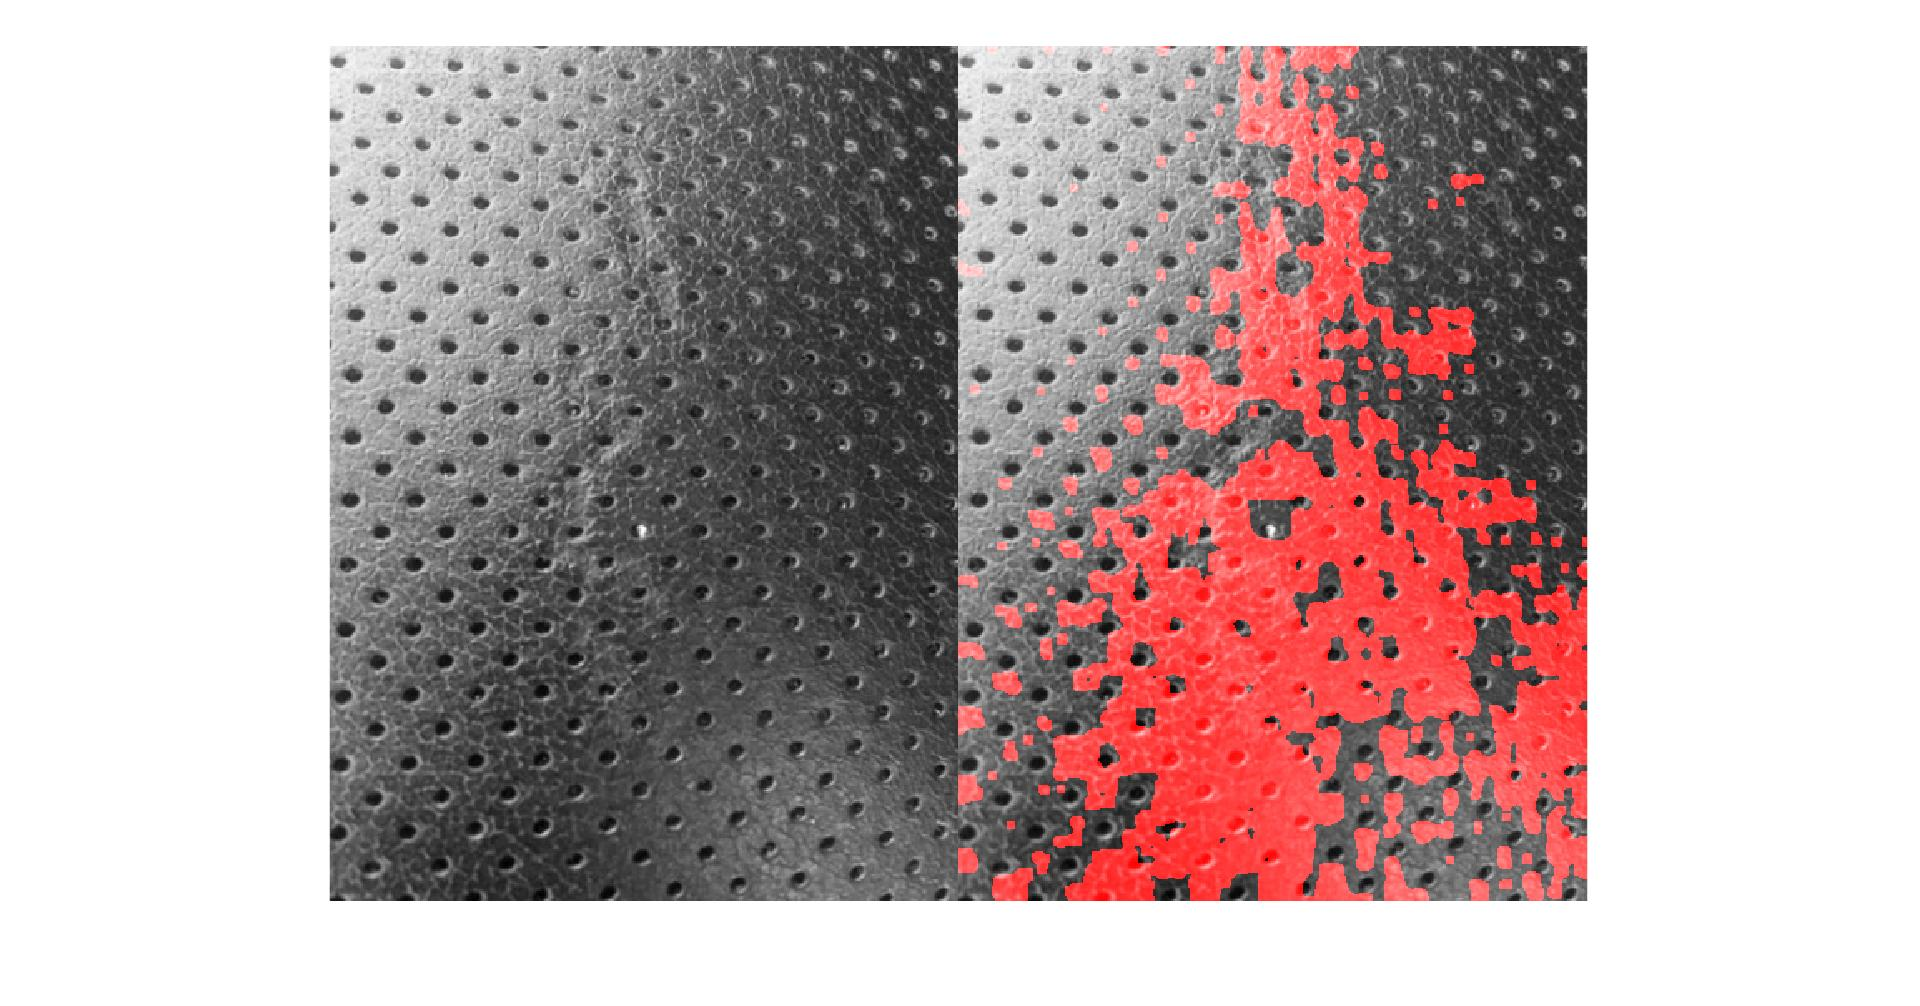
\includegraphics[width=\textwidth]{results/res17.jpg}
	\caption{Tessitura 17}
\end{figure}

Presenta gli stessi problemi analoghi alla figura 15 solo che alcuni angoli sono più chiari mentre altri sono più scuri.

\subsection{Tessitura 18}

\begin{figure}[h!]
	\centering
	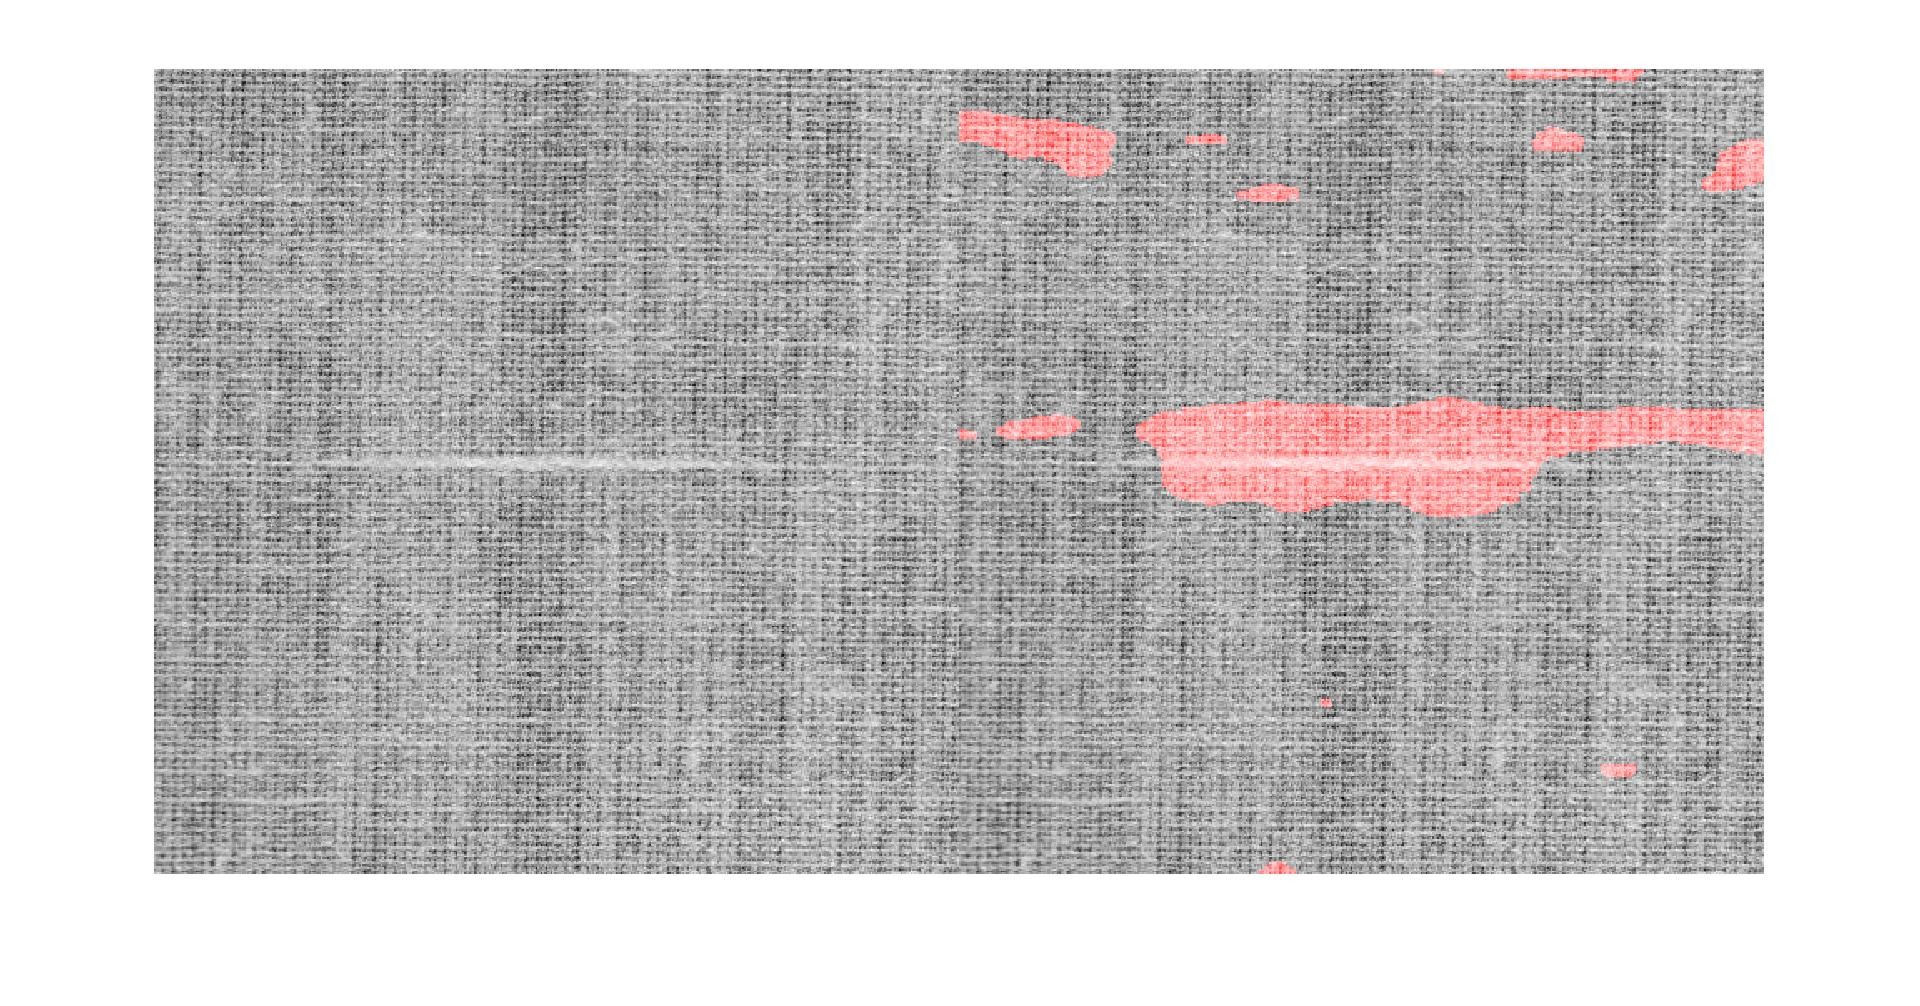
\includegraphics[width=\textwidth]{results/res18.jpg}
	\caption{Tessitura 18}
\end{figure}

\subsection{Tessitura 19}

\begin{figure}[h!]
	\centering
	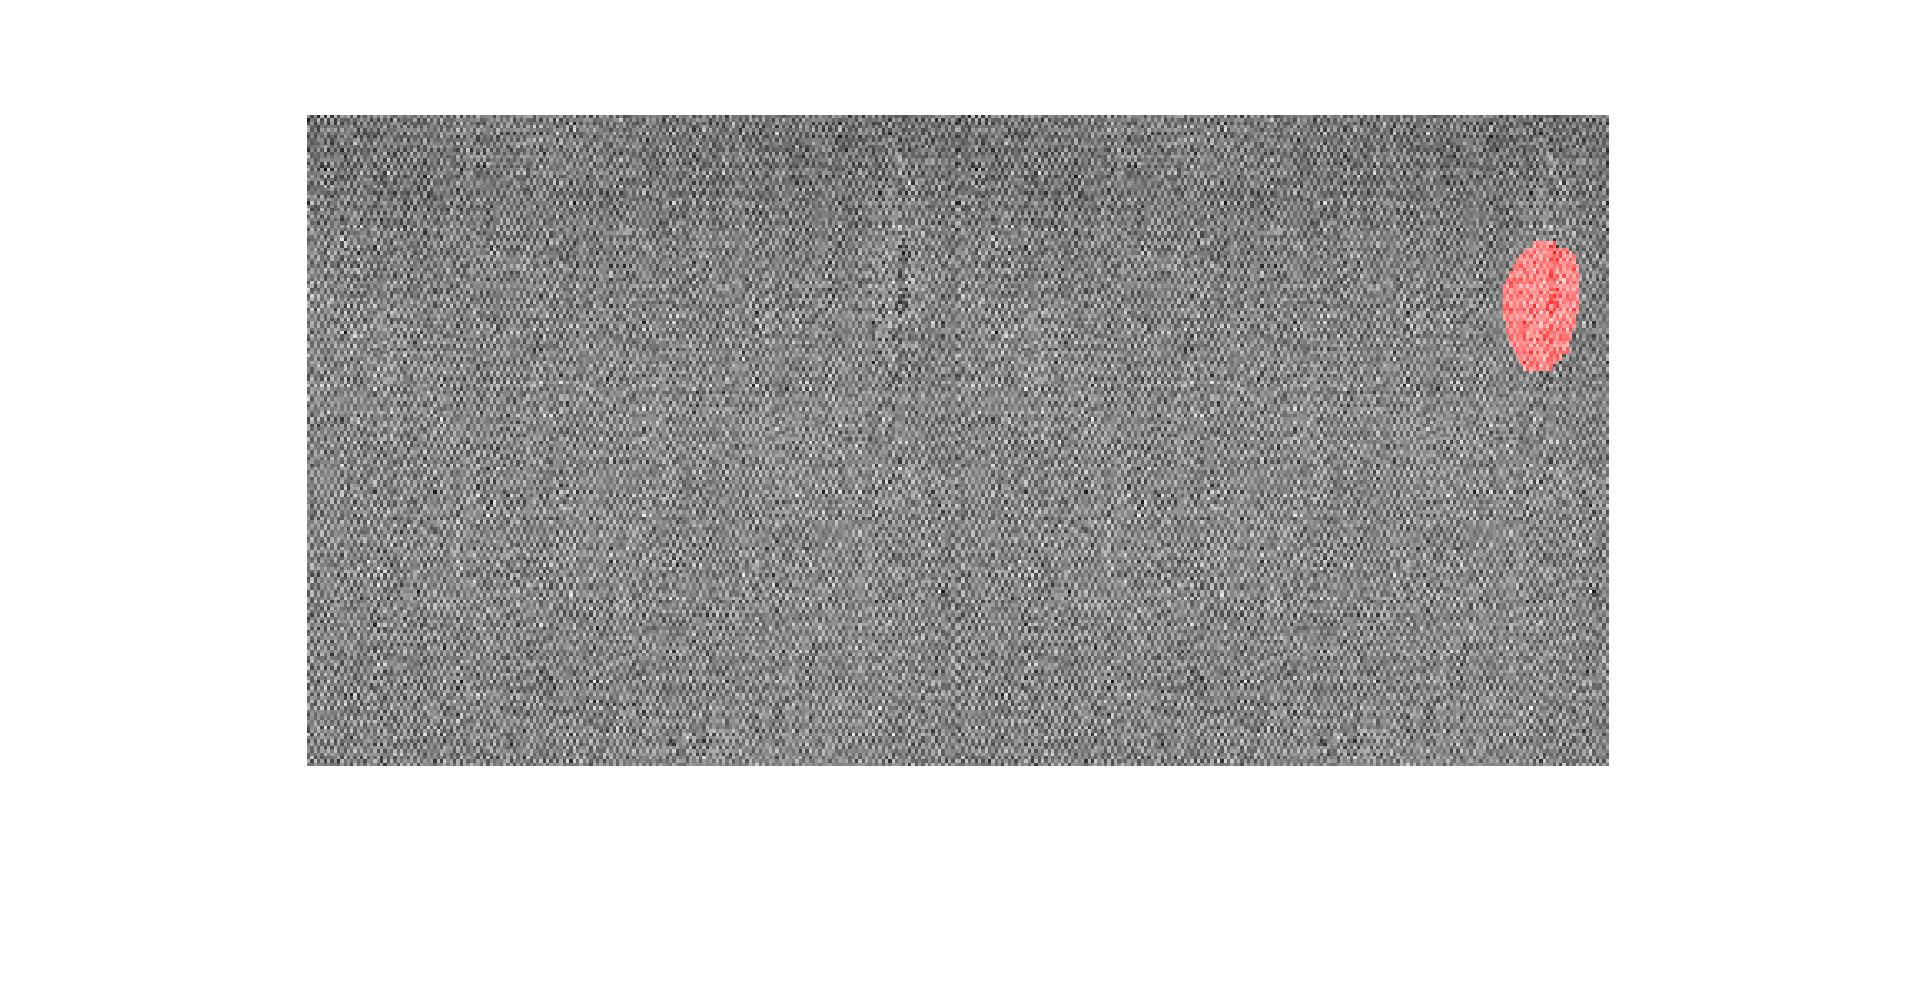
\includegraphics[width=\textwidth]{results/res19.jpg}
	\caption{Tessitura 19}
\end{figure}

\subsection{Tessitura 20}

\begin{figure}[h!]
	\centering
	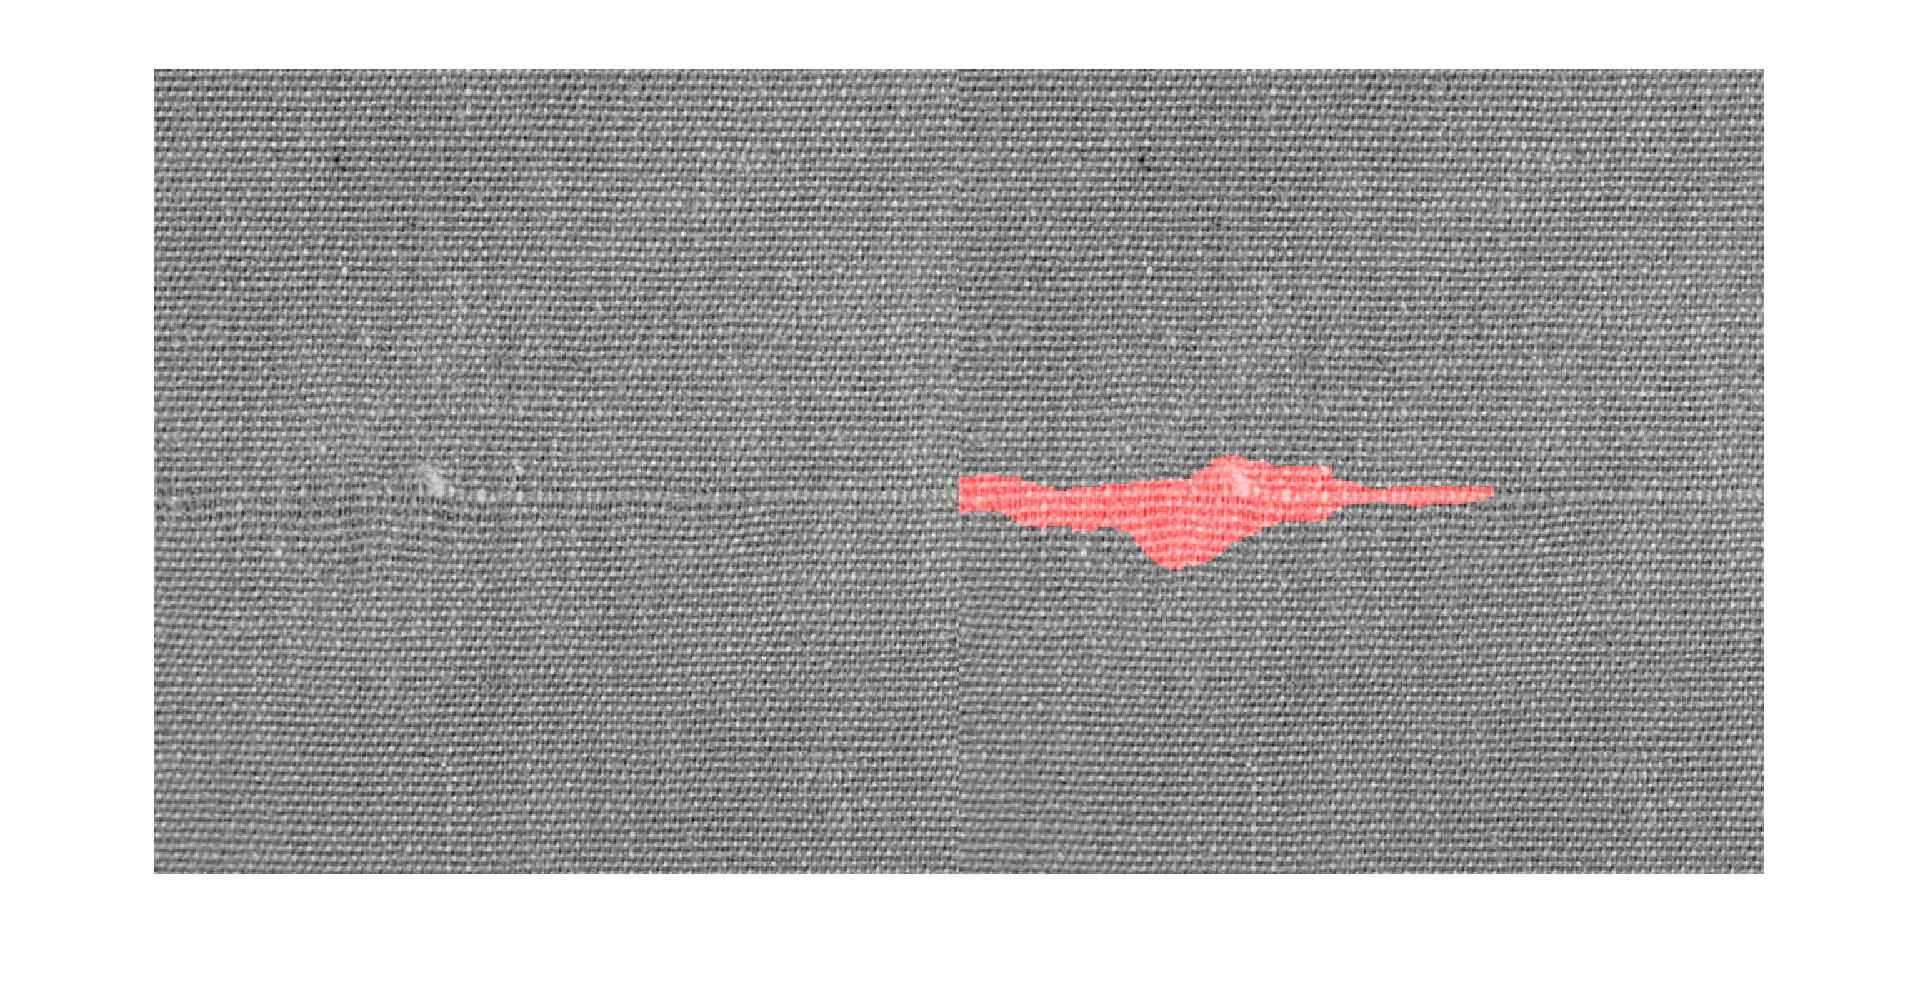
\includegraphics[width=\textwidth]{results/res20.jpg}
	\caption{Tessitura 20}
\end{figure}

\newpage

\subsection{Tessitura 21}

\begin{figure}[h!]
	\centering
	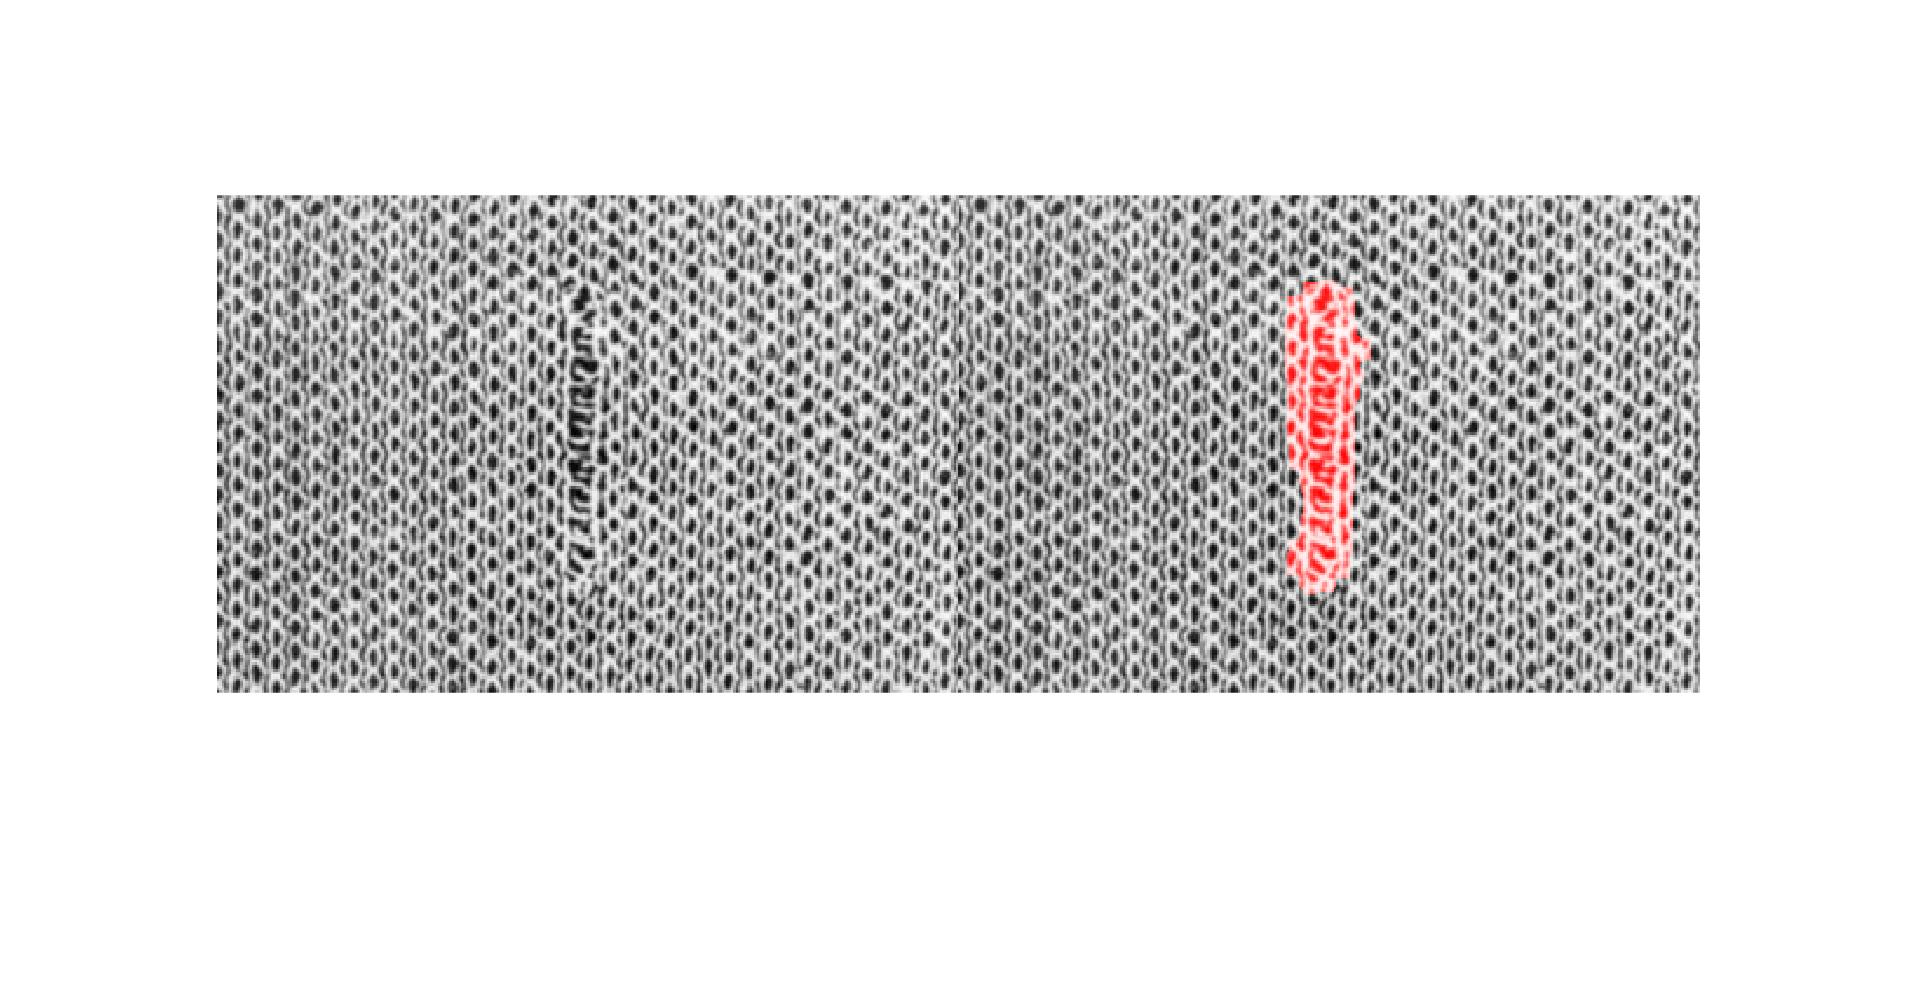
\includegraphics[width=\textwidth]{results/res21.jpg}
	\caption{Tessitura 21}
\end{figure}


\subsection{Tessitura 22}

\begin{figure}[h!]
	\centering
	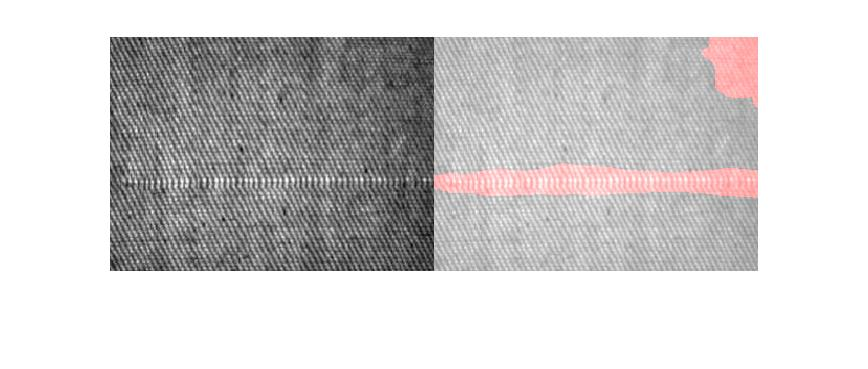
\includegraphics[width=\textwidth]{results/res22.jpg}
	\caption{Tessitura 22}
\end{figure}

\newpage

\subsection{Tessitura 23}

\begin{figure}[h!]
	\centering
	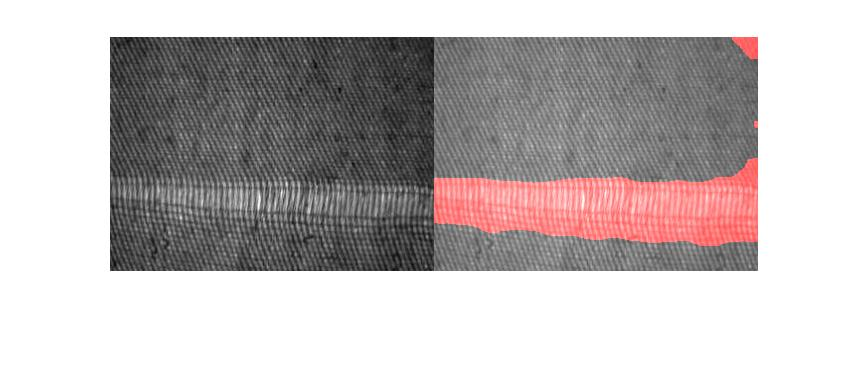
\includegraphics[width=\textwidth]{results/res23.jpg}
	\caption{Tessitura 23}
\end{figure}


\subsection{Tessitura 24}

\begin{figure}[h!]
	\centering
	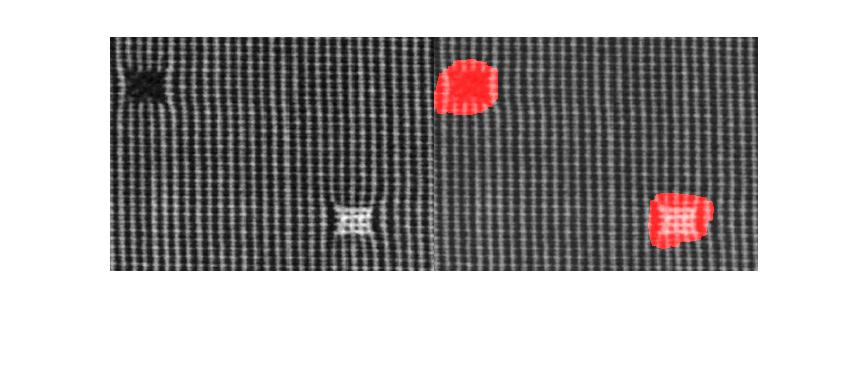
\includegraphics[width=\textwidth]{results/res24.jpg}
	\caption{Tessitura 24}
\end{figure}

\newpage

\subsection{Tessitura 25}

\begin{figure}[h!]
	\centering
	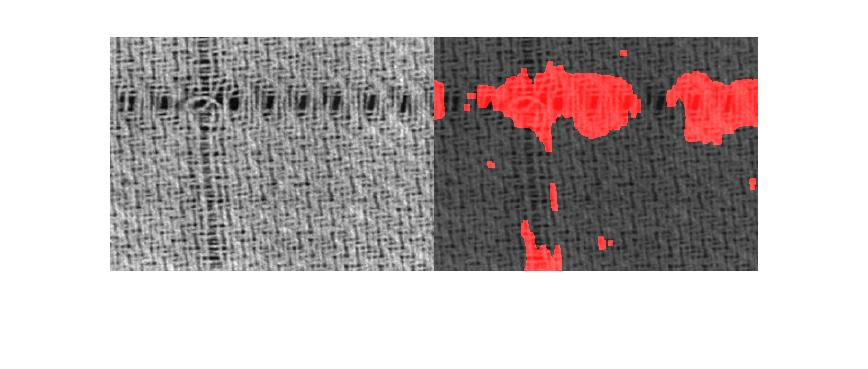
\includegraphics[width=\textwidth]{results/res25.jpg}
	\caption{Tessitura 25}
\end{figure}


\subsection{Tessitura 26}

\begin{figure}[h!]
	\centering
	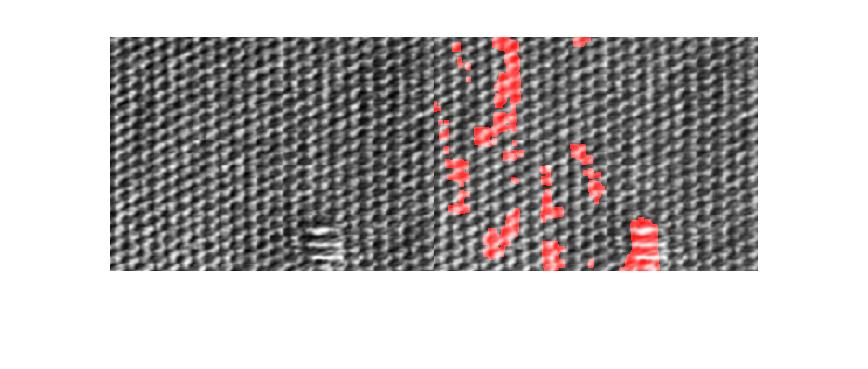
\includegraphics[width=\textwidth]{results/res26.jpg}
	\caption{Tessitura 26}
\end{figure}

\newpage

\subsection{Tessitura 27}

\begin{figure}[h!]
	\centering
	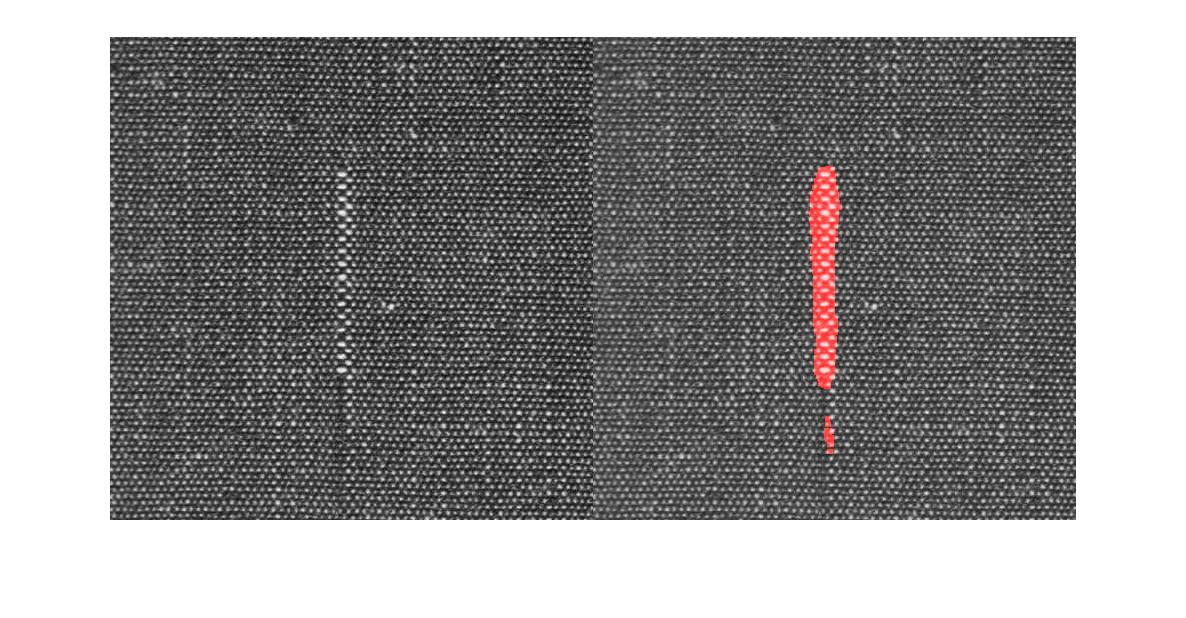
\includegraphics[width=\textwidth]{results/res27.jpg}
	\caption{Tessitura 27}
\end{figure}


\subsection{Tessitura 28}

\begin{figure}[h!]
	\centering
	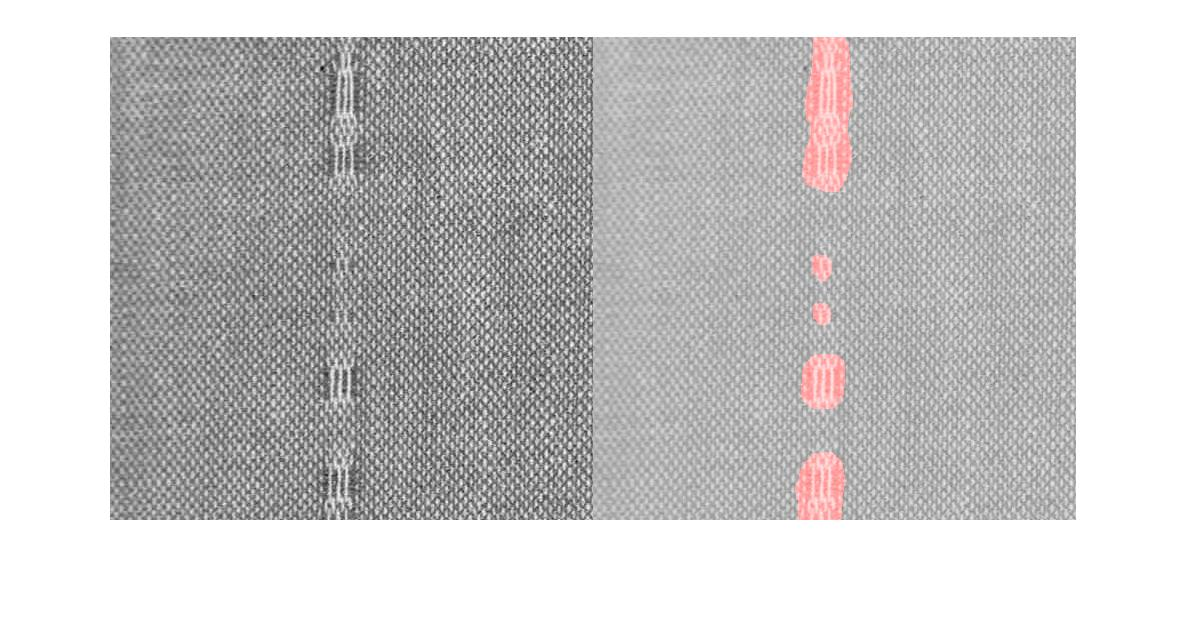
\includegraphics[width=\textwidth]{results/res28.jpg}
	\caption{Tessitura 28}
\end{figure}

\newpage
\subsection{Tessitura 29}

\begin{figure}[h!]
	\centering
	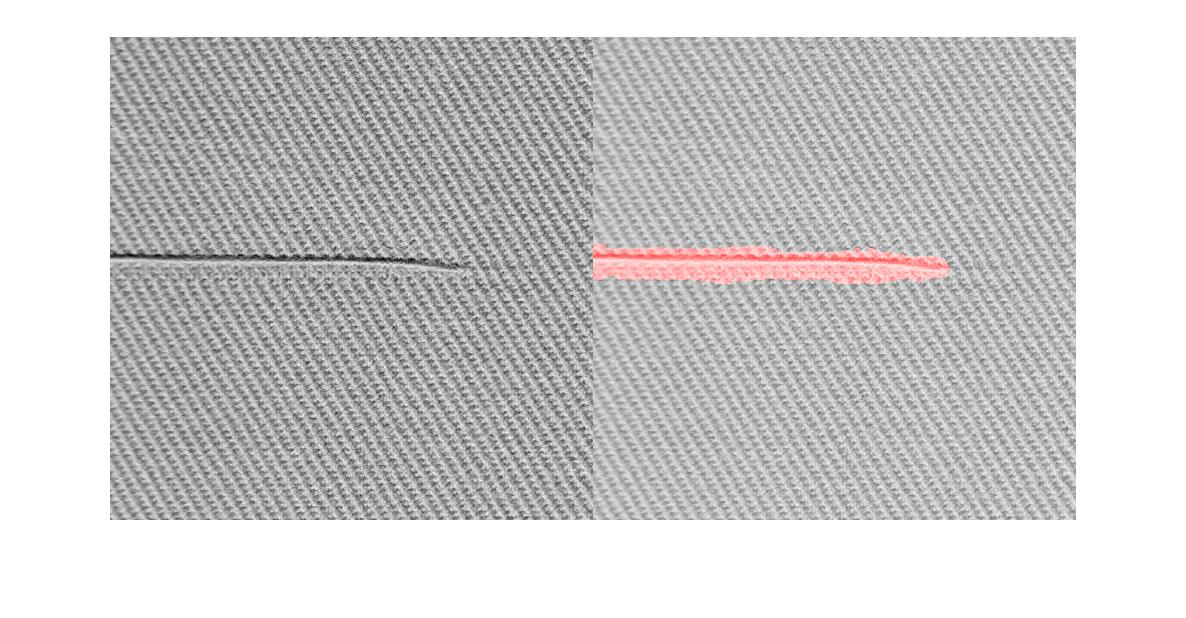
\includegraphics[width=\textwidth]{results/res29.jpg}
	\caption{Tessitura 29}
\end{figure}


\subsection{Tessitura 30}

\begin{figure}[h!]
	\centering
	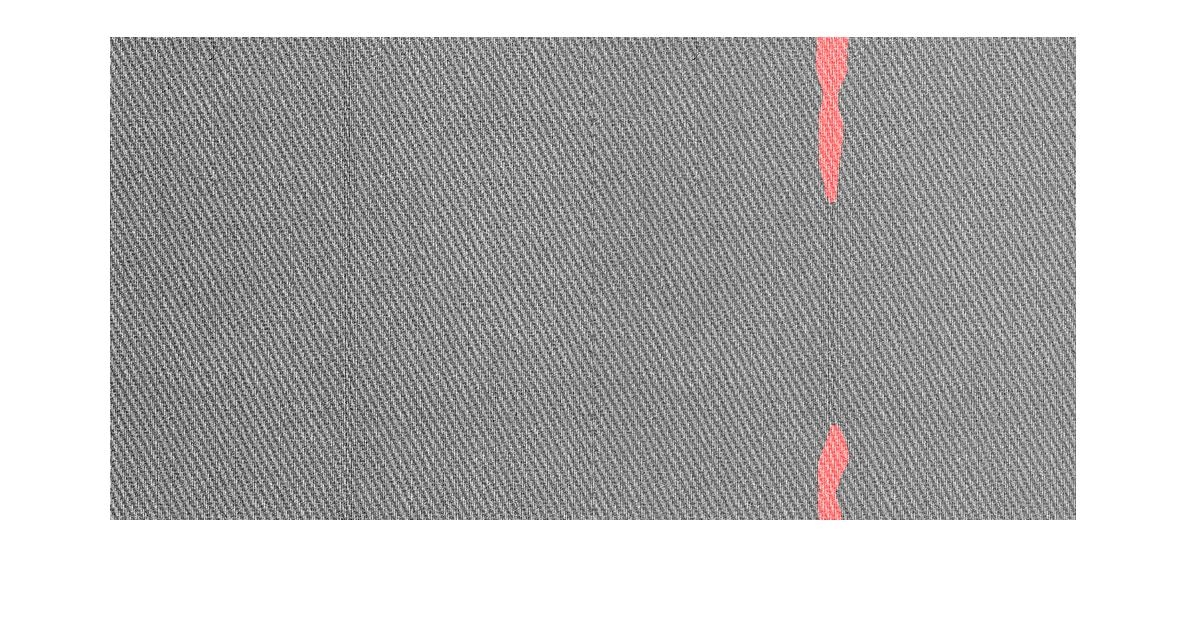
\includegraphics[width=\textwidth]{results/res30.jpg}
	\caption{Tessitura 30}
\end{figure}

\newpage
\subsection{Tessitura 31}

\begin{figure}[h!]
	\centering
	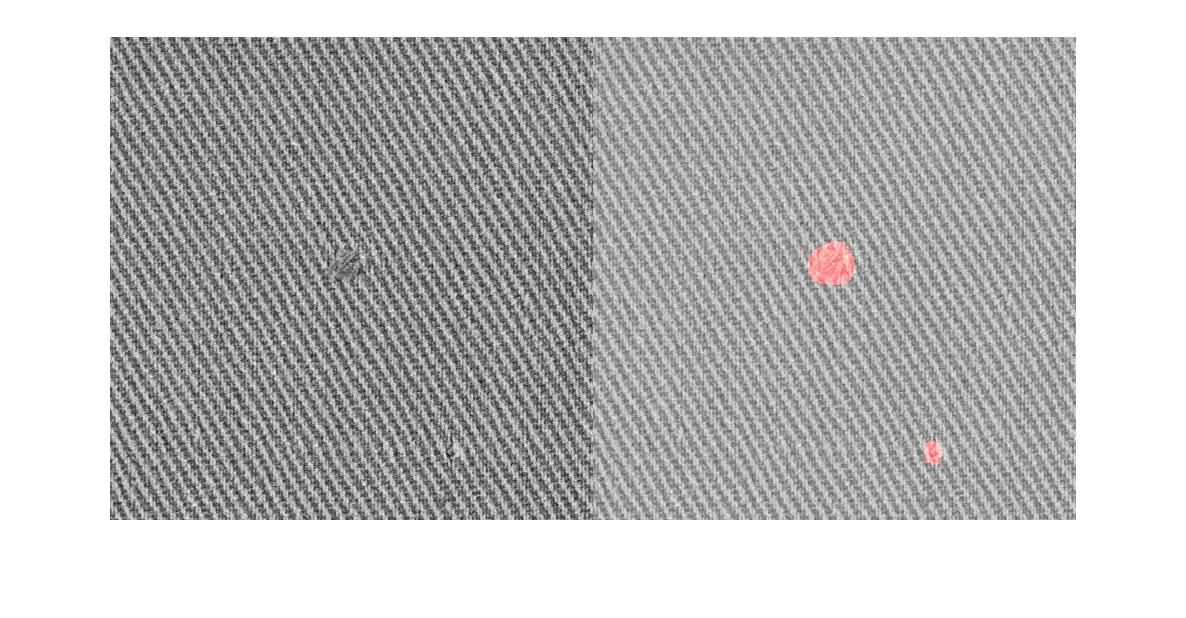
\includegraphics[width=\textwidth]{results/res31.jpg}
	\caption{Tessitura 31}
\end{figure}


\subsection{Tessitura 32}

\begin{figure}[h!]
	\centering
	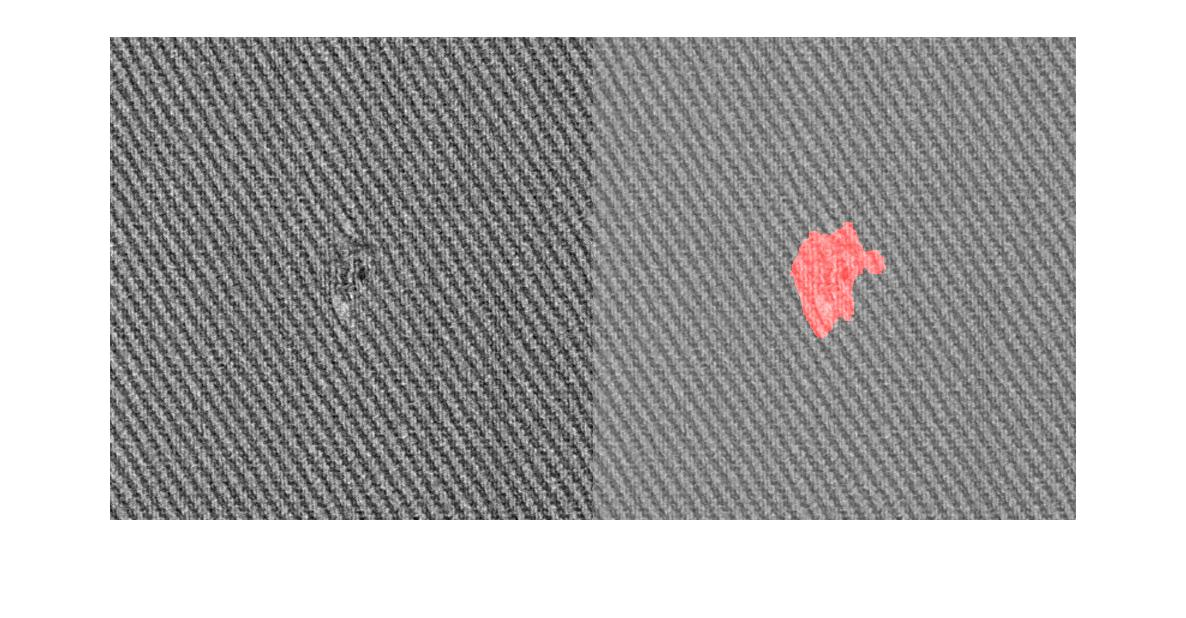
\includegraphics[width=\textwidth]{results/res32.jpg}
	\caption{Tessitura 32}
\end{figure}

\newpage


\section{Ulteriori prove fatte}

\subsection{Operazioni sull'istogramma dell'immagine di input}

Nel tentativo di migliorare il risultato della cross-correlazione sono stati applicati
equalizzazione e stretching dell'istogramma, ma sembra che non apportino nessun beneficio
evidente.

\subsection{Modifiche dei pattern usati nella cross-correlazione}

\begin{itemize}
  \item Dimensione del pattern variabile e proporzionale alla dimensione dell'immagine di input:
  
  Data la dimensione delle immagini di input variabile abbiamo provato a rendere la
  dimensione dei pattern proporzione alla grandezza dell'immagine, ma sembra non avere alcun
  vantaggio evidente.
  Però introducendo la possibilità di variare la grandezza dei pattern a piacimento ci ha permesso 
  di risolvere il problema delle immagini con disegni particolari (vedi fig. 4).

  \item Numero di pattern variabile:
  
  Durante le prove abbiamo introdotto la possibilità di aumentare a piacimento il numero di
  pattern, ma da un certo punto in poi aumentarne il numero diventa solo uno spreco di risorse
  di computazione senza variare il risultato.
  
  \item Posizione dei pattern random:
  
  Il problema di questa funzionalità è che il risultato finale dell'elaborazione cambia ad ogni
  esecuzione.
  Inoltre ogni volta che vengono applicate modifiche al codice, per esempio viene introdotto un
  nuovo filtro, non siamo in grado di capire il vero effetto apportato dalle modifiche data dal
  fatto che il risultato cambia per ogni esecuzione.
  Un altro problema si presenta quando il pattern generato casualmente si trova in una zona in cui è situato un difetto e quindi non è considerabile come campione valido per il calcolo della cross-correlazione.
  
  
\end{itemize}

\subsection{Filtri di sharpening sull'immagine di input}

Un altro tentativo di migliorare il risultato della cross-correlazione è stata l'applicazione di un filtro laplaciano all'immagine originale, per rendere
più evidenti i bordi, ma sembra che ciò non abbia effetto sul risultato della cross-correlazione
applicata successivamente.

\subsection{Filtri sull'immagine di cross-correlazione}

Applichiamo questi filtri alla cross-correlazione per migliorare il calcolo della soglia di
binarizzazione, dopo aver provato vari filtri come quello di media, mediana, deviazione standard,range filter e filtro gaussiano. Siamo arrivati alla conclusione che il filtro di deviazione
standard fornisce il risultato migliore.

\subsection{Operazioni sull'istogramma dell'immagine di cross-correlazione}

Applichiamo le operazioni di equalizzazione e stretching dell'istogramma della cross-correlazione nel tentativo di migliorare il calcolo della soglia di binarizzazione.
Non hanno apportato alcun miglioramento causa la natura dell'algoritmo di binarizazione di Otsu
utilizzato.

\subsection{Analisi in frequenza 2D}

Abbiamo provato a rimuovere la tessitura per migliorare l'individuazione dei difetti.
Applicando la trasformata di Fourier 2D sulle immagini abbiamo notato che esse presentano dei
picchi irregolari e non particolarmente elevati pertanto risulta difficile identificarli.
Le immagini che producono una trasformata migliore sono quelle dove vi è un pattern ben 
definito, ad esempio le figure 4, 10, 15 e 17.

Abbiamo effettuato delle prove manuali nella rimozione di questi picchi, ma non ci hanno portato ad un risultato soddisfacente.

\newpage

\end{document}